\newcommand{\electronic}[2]{#2} % #1 = printer friendly version, #2 = screen viewing version

\electronic{\documentclass[article]{memoir}}{\documentclass[article,openany]{memoir}}

\usepackage{amsmath,amssymb, amsthm}
\usepackage[usenames,dvipsnames]{xcolor}
\definecolor{darkgreen}{rgb}{0,0.5,0}
\definecolor{darkblue}{rgb}{0,0,0.5}
\electronic{\usepackage[colorlinks=true,urlcolor=black,citecolor=black,linkcolor=black]{hyperref}}{\usepackage[colorlinks=true,urlcolor=darkblue,citecolor=darkgreen,linkcolor=darkblue]{hyperref}}

\usepackage{bbm}
\usepackage[latin1]{inputenc}
\usepackage[T1]{fontenc}
\usepackage{lmodern}
\usepackage{graphicx}
\usepackage[all,cmtip]{xy}

\electronic{\setlrmarginsandblock{*}{4.0cm}{0.75}}{\setlrmarginsandblock{*}{3.5cm}{1}}
\setulmarginsandblock{3.0cm}{*}{1.2}
\checkandfixthelayout

\renewcommand{\bibname}{References}

\newcommand{\word}[1]{#1\index{#1}}
\newcommand{\emphword}[1]{\emph{#1}\index{#1}}

\newcommand{\relmiddle}[1]{\mathrel{}\middle#1\mathrel{}}

\newcommand{\abs}[1]{\lvert #1 \rvert}
\newcommand{\Abs}[1]{\lVert #1 \rVert}

\newcommand{\bbR}{\mathbb{R}}
\newcommand{\bbC}{\mathbb{C}}
\newcommand{\bbN}{\mathbb{N}}
\newcommand{\bbQ}{\mathbb{Q}}
\newcommand{\bbZ}{\mathbb{Z}}

\newcommand{\calT}{\mathcal{T}}

\newcommand{\eps}{\varepsilon}
\renewcommand{\epsilon}{\varepsilon}
\renewcommand{\phi}{\varphi}

\theoremstyle{plain}
\newtheorem{lem}{Lemma}[chapter]
\newtheorem{thm}[lem]{Theorem}
\newtheorem{prop}[lem]{Proposition}
\newtheorem{cor}[lem]{Corollary}

\theoremstyle{definition}
\newtheorem{defn}[lem]{Definition}
\newtheorem{example}[lem]{Example}

\theoremstyle{remark}
\newtheorem{rem}[lem]{Remark}

\makechapterstyle{combined}{
  \setlength{\midchapskip}{10pt}
  \setlength{\afterchapskip}{2.5cm}
  \renewcommand*{\printchaptername}{}
  \renewcommand*{\chapnumfont}{\normalfont\sffamily\bfseries\fontsize{42}{0}\selectfont}
  \renewcommand*{\printchapternum}{\flushright\normalfont\sffamily\Huge\bfseries Chapter \chapnumfont{\thechapter}}
  \renewcommand*{\chaptitlefont}{\normalfont\sffamily\bfseries\Huge}
  \renewcommand*{\printchaptertitle}[1]{\bfseries\chaptitlefont{##1}}
    %\raggedright\chaptitlefont\parbox[t]{\textwidth}{\raggedright##1}}
}
\chapterstyle{combined}

\renewcommand{\secheadstyle}{\sffamily\LARGE\bfseries}
\renewcommand{\subsecheadstyle}{\sffamily\Large\bfseries}
\counterwithout{section}{chapter}
\setsecnumdepth{subsection}
\setcounter{tocdepth}{2}

\makeindex
\begin{document}

\frontmatter

\pretitle{\begin{center}\Huge\bfseries}
\title{Basic topology}
\posttitle{\par\vskip1em{\normalfont\normalsize\scshape Lecture notes for a 2015 Uppsala University course\par\vfill}\end{center}}
\author{S{\o}ren Fuglede J{\o}rgensen}
\predate{\vfill\begin{center}\large Version: }

\begin{titlingpage}
\maketitle
\end{titlingpage}


\tableofcontents

\section{Preface}
\label{preface}
These are lecture notes written for a course on elementary point set topology given at Uppsala University during the spring of 2015. The notes are, at the time of writing, \emph{not} intended as a full reference for the course. Rather, the course will follow the references \cite{Mun} and \cite{Fje}, and these notes serve to show which parts of the main references we have covered in the lectures.

The notes will be written as the course moves along and may be discontinued at any moment, depending on time restrictions. As such, they are also likely to contain typos and errors of other kinds; if you come across any such, feel very free to let me know, either by email at \href{mailto:s@fuglede.dk}{\textsf{s@fuglede.dk}}, or by letting me know in person. Concrete changes can also be proposed directly at \url{https://github.com/fuglede/basic-topology}.

\subsection{Terms of use}
Whenever applicable, this text is licensed under the Creative Commons Attribution-ShareAlike 4.0 International License. To view a copy of this license, visit \url{https://creativecommons.org/licenses/by-sa/4.0/}. Some parts of the text will originate from other sources; in these cases the relevant terms have been included.


\section{Introduction}
\label{introduction}
This course will mainly be concered with the study of topological spaces. Topological spaces are abstract mathematical concepts whose definition include a sufficient amount of data for them to be called ``spaces''. Familiar spaces would be something like $\mathbb{R}^3$ or $\mathbb{R}^n$, but more abstract objects -- such as general vector spaces -- we also think of as ``spaces''. On the other hand, in algebra one encounters objects such as groups and rings that one would generally not think of as spaces, and on the extreme side we talk about sets, which are more general ``collections of things'' which we may or may not choose to think of as spaces.

From this point of view, one might think of topological spaces with an added bit of \word{structure}{struktur}\footnote{See \url{https://en.wikipedia.org/wiki/Mathematical_structure} for a more precise discussion.}; a term used throughout mathematics but typically with a rather vague meaning. As such, sets have no interesting structure, but Euclidian space $\mathbb{R}^n$ has plenty: for instance, the usual inner product $\langle \cdot ,\cdot \rangle$ on $\mathbb{R}^n$ can be used to talk about angles between vectors. This in turn can be used to define the standard norm $\lVert \cdot \rVert$ on $\mathbb{R}^n$ which allows us to talk about lengths of vectors and distances between points. All of this is structure that may not be given to us in a general vector space, but without having this structure on $\mathbb{R}^n$, there would be no such thing as calculus: we wouldn't be able to define things like differentiability and continuity.

For topological spaces we discard all of this fine structure, so that in particular it makes no sense to talk about the distance between two points in a general topological space. The only piece of structure that we will require is that of ``open sets'': given a subset of a topological space, we want to be able to tell if it is open or not. This turns out to be the least amount of structure needed to define continuity, so the study of topological spaces is very much the study of continuous functions.

The study of general topological spaces and continuous functions will be contained in Sections~\ref{topological-spaces}--\ref{homeomorphisms}. Simply having open sets turns out also to be sufficient to talk about what it means for a space to be ``connected'' and ``compact'' in a way that corresponds to what one would normally associate with those words. More abstractly, we will also look at the notion of separating points, which is less familiar in examples like $\mathbb{R}^n$. These properties of topological spaces will be the basis of Sections~\ref{connectedness}--\ref{separation}.

The study of general topological spaces and their fundamental properties is often referred to as \word{point-set topology}{?} or \word{general topology}{?}. The less structure a certain space has, the less deep the mathematical results about it tends to be, and out treatment will involve correspondly few deep mathematical theorems; rather, for the first part of the course, one should think of the materials as developing the necessary tools to deal with topological spaces in other contexts. Towards the end of the course, we will remedy this by tying together our theory with other parts of mathematics. Concretely, in Section~\ref{homotopy} we touch upon the mathematical area of \word{algebraic topology}{algebraisk topologi} which is concerned with analyzing certain natural algebraic structures that can be associated with topological spaces, and in Section~\ref{manifolds}, we will study a particular nice family of topological spaces called manifolds that show up in all of geometry.

Before being able to do any of this, though, we need to firmly settle on what sets are, and how one deals with them.


\mainmatter

\section{Set theory and logic}
\label{set-theory}

The theory of sets, typically referred to as \word{set theory}{m{\"a}ngdteori}, forms the basic fundament of all of mathematics. As such, it is probably unsurprising that a huge body of work has been devoted to it. This, however, is not obvious if one simply reads these notes as we will not at all deal with many of the important ideas that underly the theory. Moreover, even though set theory plays an essential role in our study, our treatment of set theory will be rather brief, so the inexperienced reader is also strongly encouraged to study \cite[\S1]{Mun} in detail.

\subsection{Basic notions}
Whereas everything that we will during the course will be as mathematically precise as one can get, we will begin by imprecisely considering a \word{set}{m{\"a}ngd} as a ``collection of things''. These ``things'' will be referred to as the \emph{elements} of the set.

If $A$ is a set, and $a$ is an element of $A$, we write
\[
  a \in A.
\]
Synonymously, we will sometimes say that $a$ is contained in $A$. If on the other hand $a$ is not an element of $A$, then we write
\[
  a \notin A.
\]
If $B$ is another set which contains all the elements of $A$; that is, if $a \in A$ implies that $a \in B$, then we say that $A$ is a \word{subset}{delm{\"a}ngd} of $B$ and write
\[
  A \subset B.
\]
We will also sometimes say that $A$ is contained in $B$ or that $B$ contains $A$. If $A \subset B$ but $A \not= B$, we will write
\[
  A \subsetneq B
\]
and say that $A$ is a \word{proper subset}{{\"a}kta delm{\"a}ngd} of $B$. Set-theoretic relationships are often depicted in so-called Euler diagrams; see Figure~\ref{eulersubset}.
\begin{figure}
  \centering
  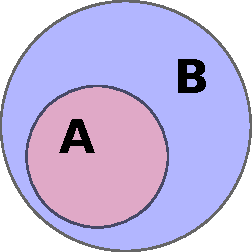
\includegraphics{images/subset.pdf}
  \caption{The Euler diagram representing the inclusion $A \subset B$.}
  \label{eulersubset}
\end{figure}
\begin{example}
  When a set contains only very few elements, one simply lists them. For instance, if $A$ contains only the elements $a$ and $b$, we write $A = \{ a, b\}$. Then if $B = \{ a, b, c\}$, we see for instance that $A \subset B$ and since $c \in B$ but $c \notin A$, we have that $A \not= B$, so $A \subsetneq B$.
  
  Often, sets are given by the properties of their elements, and this will be built into our notation. For instance, the set containing the even numbers will be written
  \[
    \{ x \mid \text{$x$ is an even integer} \},
  \]
  which should be read as ``$x$ such that $x$ is an even integer''.
  
  We will also often be considering the set which contains no elements at all; this set is called \word{the empty set}{den tomma m{\"a}ngden} and is denoted $\emptyset$. This has the property that $\emptyset \subset X$, no matter what $X$ is.
\end{example}
\begin{defn}
  Let $X$ be any set. The \word{power set}{potensm{\"a}ngd} of $X$, denoted $\calP(X)$ is the set of all subsets of $X$, that is
  \[
    \calP(X) = \{U \mid U \subset X \}.
  \]
\end{defn}
\begin{example}
  The elements of power sets are themselves sets which in turn may also have elements. Some examples of power sets are the following:
  \begin{align*}
    \calP(\{a\}) &= \{ \emptyset, \{a \} \}, \\
    \calP(\{a,b\}) &= \{ \emptyset, \{a\}, \{b\} , \{a,b\} \}.
  \end{align*}
  In general, if $X$ is a finite set containing $n$ elements, then $\calP(X)$ contains $2^n$ elements. The only subset of $\emptyset$ is $\emptyset$ itself, which means that
  \[
    \calP(\emptyset) = \{\emptyset\}.
  \]
  Be aware that $\{ \emptyset \}$ consists of a single element, namely $\emptyset$, so $\{\emptyset\}$ is not itself empty, even though it is tempting to read the notation like that.
\end{example}
\begin{defn}
  Given two sets $A$ and $B$, we define their \word{union}{union} $A \cup B$ and \word{intersection}{snitt} $A \cap B$ as
  \begin{align*}
    A \cup B = \{ x \mid \text{$x \in A$ or $x \in B$} \}, \\
    A \cup B = \{ x \mid \text{$x \in A$ and $x \in B$} \}. \\
  \end{align*}
  The sets $A$ and $B$ are called \word{disjoint}{disjunkt} if $A \cap B = \emptyset$. We also introduce the \word{difference}{differens} $A \setminus B$, or sometimes $A - B$, given by
  \[
    A \setminus B = \{ x \mid \text{$x \in A$ and $x \notin B$} \}.
  \]
  If $A \subset X$ for some set $X$, we introduce the \word{complement}{komplement} of $A$, written $A^c$ as
  \[
    A^c = X \setminus A.
  \]
  Note that $X$ does not feature in the notation for complements but which set it is will always be clear from the context. See Figure~\ref{union-intersection} for the corresponding Euler diagrams.
\end{defn}
\begin{figure}
  \centering
  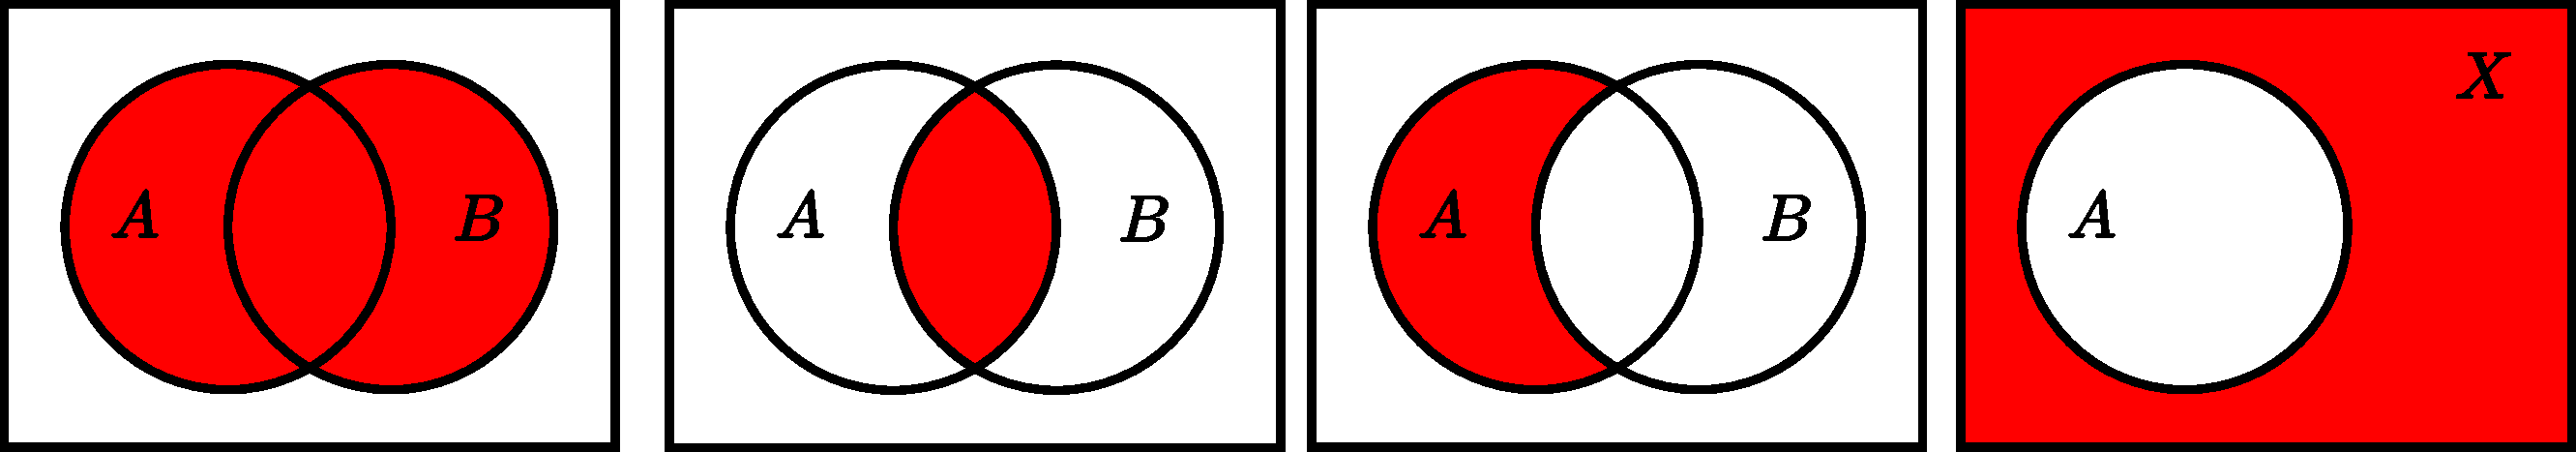
\includegraphics[scale=0.3]{images/union-intersection.pdf}
  \caption{The red sets illustrate $A \cup B$, $A \cap B$, $A \setminus B$, and $A^c$ respectively.}
  \label{union-intersection}
\end{figure}

\subsection{Set theory and boolean logic}
At this point, let us remark that sets and their operations closely mimic logical statements and their boolean logic, and without making this statement too precise, one could summarize their relationship in the following table:

\begin{center}
\begin{tabular}{ccc}
  logic & English & set theory \\
  \hline
  $P \Rightarrow Q$ & $P$ implies $Q$ & $A \subset B$ \\
  $P \Leftrightarrow Q$ & $P$ is equivalent to $Q$ & $A = B$ \\
  $P \vee Q$ & $P$ and $Q$ & $A \cup B$ \\
  $P \wedge Q$ & $P$ or $Q$ & $A\cap B$ \\
  $\neg P$ & not $P$ & $A^c$
\end{tabular}
\end{center}

For convenience, and for those who may not have encountered boolean logic before, we recall that these logical operations are defined through truth tables. Here, $P$ and $Q$ are statements that may be either true (T) or false (F), and the values of $P \Rightarrow Q$, $P \Leftrightarrow Q$, etc., are defined accordingly:
\begin{center}
\begin{tabular}{c|c}
  $P$ & $\neg P$ \\
  \hline
  T & F \\
  F & T
\end{tabular}
\quad \quad
\begin{tabular}{cc|cc}
  $P$ & $Q$ & $P \wedge Q$ & $P \vee Q$ \\
  \hline
  T & T & T & T \\
  T & F & F & T \\
  F & T & F & T \\
  F & F & F & F
\end{tabular}
\end{center}

In these tables, the columns to the left of the vertical bar are the assumptions, and the columns to the right are the definitions. Armed with these definitions, one simply defines $P \Rightarrow Q$ as $\neg P \vee Q$, and similarly $P \Leftrightarrow Q$ is defined as $(P \Rightarrow Q) \vee (Q \Rightarrow P)$.

With these, one sees that the correspondence in the first table in this section is obtained when $P$ is the statement $a \in A$, and $Q$ is the statement $a \in B$.

\subsection{Arbitrary unions and intersections}
So far, we have considered only operations on pairs of sets, but more often than not we will be dealing with infinite families of sets. First of all, we introduce the notation $\forall$ meaning ``for all'', and $\exists$ meaning ``there exists''.

Let $I$ is any set. Then a collection $\{ A_i \}_{i \in I}$ of sets $A_i$ is called a family of sets parametrised by $I$. For such a family, define the infinite union, and the infinite intersection as
\begin{align*}
  \bigcup_{i \in I} A_i &= \{ x \mid \text{$\exists i \in I$ such that $x \in A_i$} \},\\
  \bigcap_{i \in I} A_i &= \{ x \mid \text{$x \in A_i \ \forall i \in I$} \}.
\end{align*}
It might be helpful to compare these definitions with the definitions of union and intersection from above, which is the case where $I$ contains two elements.

\begin{prop}
  For sets $A$, $B$, $C$, and $X$, for a family $\{ A_i \}_{i \in I}$ with $A_i \subset X$ for all $i \in I$, one has the useful identities,
  \begin{align*}
    A \cap (B \cup C) &= (A \cap B) \cup (A \cap C), \\
    A \cup (B \cap C) &= (A \cup B) \cap (A \cup C), \\
    X \setminus \bigcup_{i \in I} A_i &= \bigcap_{i \in I} X \setminus A_i, \\
    X \setminus \bigcap_{i \in I} A_i &= \bigcup_{i \in I} X \setminus A_i.
  \end{align*}
\end{prop}
\begin{proof}[Partial proof]
  Set theoretical identities like the above are typically shown in the same way: one starts with an element in the left hand side and proves that it is an element of the right hand side, which shows ``$\subset$'', and one then proceeds to do the same thing the other way around. To convince oneself that the identities indeed hold, it may be helpful to draw the corresponding Euler diagrams.
  
  Let us show for instance that $A \cap (B \cup C) \subset (A \cap B) \cup (A \cap C)$. To do this, let $a \in A \cap (B \cup C)$. This means that $a \in A$ and $a \in B \cup C$. The latter of these means that $a \in B$ or $a \in C$. Together, this says that either $a \in A$ and $a \in B$, or $a \in A$ and $a \in C$. Written in set notation, this says that $a \in (A \cap B) \cup (A \cap C)$.
  
  Let us also show that $X \setminus \bigcup_{i \in I} A_i \subset \bigcap_{i \in I} X \setminus A_i$. That is, let $a \in X \setminus \bigcup_{i \in I} A_i$. This says that $a \notin \bigcup_{i \in I} A_i$. From this we conclude that $a$ is not in any of the $A_i$ (since otherwise $a$ would be in their union), or in symbols, $\forall i \in I$, we have $x \notin A_i$. That is, $\forall i \in I$, we have $x \in X \setminus A_i$, but this exactly means that $x \in \bigcap_{i \in I} X \setminus A_i$.
  
  We leave the remaining six directions for the reader.
\end{proof}

\subsection{Cartesian product}
Another way of constructing new sets from old sets is through the so-called Cartesian product, often simply called a product. In words, if $A$ and $B$ are two sets, then the \word{Cartesian product}{kartesisk product, m{\"a}ngdprodukt} $A \times B$ is the set of all pairs $(a,b)$, where $a \in A$, or $b \in B$; that is,
\[
  A \times B = \{ (a,b) \mid \text{$a \in A$ and $b \in B$}\}.
\]
Be aware that $(a,b)$ is occasionally used as the notation for intervals of real numbers, but this is something completely different.

\begin{example}
  One way of defining $\bbR^2$ is simply as $\bbR^2 = \bbR \times \bbR$.
\end{example}
Just as for unions and intersections, we would like to be able to talk about infinite products. A little bit of care needs to be taken when defining these. For instance, what is $X \times Y \times Z$? There are two natural definitions: $(X \times Y) \times Z$ and $X \times (Y \times Z)$. The first set consists of elements of the form $((x,y),z)$, while the second one consists of elements of the form $(x,(y,z))$. Clearly, we should be able to think of any of these as simply triples $(x,y,z)$.

To make this precise for an infinite number of sets, consider a family $\{X_i \}_{i \in I}$. The infinite product should then consist of tuples $(x_i)_{i \in I}$ with $x_i \in X_i$ for all $i$. Such a tuple we can also view as a function $x : I \to \bigcup_{i \in I} X_i$ such that $x(i) \in X_i$ for all $i$. This brings us to the following.
\begin{defn}
  The Cartesian product of a family $\{X_i \}_{i \in I}$ is the set
  \[
    \prod_{i \in I} X_i = \left\{ x : I \to \bigcup_{i \in I} X_i \relmiddle| x(i) \in X_i \ \forall i \in I \right\}.
  \]
\end{defn}

\subsection{Relations}
Above, we have talked about various relations between sets; these we will now make mathematically precise. A \word{binary relation}{bin{\"a}r relation} $C$, often simply called a \word{relation}{relation}, on a set $A$ is a subset $C \subset A \times A$. When $(x,y) \in C$, we will often write $xCy$.

\begin{example}
  \label{example-inequality}
  The subset of $\bbR \times \bbR$ given by $C = \{(x,y) \mid x \leq y\}$ is a relation on $\bbR$, and $xCy$ if and only if $x \leq y$.
\end{example}

\begin{defn}
  A relation $C \subseteq A \times A$ is called
  \begin{itemize}
    \item \word{reflexive}{reflexiv} if $xCx$ for all $x \in A$,
    \item \word{symmetric}{symmetrisk} if $xCy$ implies that $yCx$ for all $x,y \in A$,
    \item \word{anti-symmetric}{antisymmetrisk} if $xCy$ and $yCx$ implies that $x = y$ for all $x, y \in A$,
    \item \word{transitive}{transitiv} if $xCy$ and $yCz$ implies that $xCz$ for all $x,y,z \in A$,
    \item \word{total}{total} if either $xCy$ or $yCx$ when $x, y \in A$.
  \end{itemize}
\end{defn}
\begin{example}
  The relation $\leq$ from Example~\ref{example-inequality} is reflexive, anti-symmetric, transitive, and total, but it is not symmetric.
\end{example}
\begin{defn}
  A relation $C$ on a set $A$ is called a \word{partial order}{partiell ordning} if it is reflexive, anti-symmetric, and transitive. The pair $(A,C)$ is called a \word{poset}{pom{\"a}ngd}.
\end{defn}
\begin{defn}
  An \word{equivalence relation}{ekvivalensrelation} is a relation which is reflexive, symmetric, and transitive.
\end{defn}
When $C$ is an equivalence relation, we will use the notation $x \sim y$ for $xCy$ and say that $x$ is equivalent to $y$.
\begin{example}
  \label{congruence}
  Fix a positive integer $p \in \bbN$, and let $C \subset \bbZ \times \bbZ$ be the subset of pairs $(m,n)$ such that $m-n$ is a multiple of $p$, i.e. $m-n = dp$ for some $d \in \bbZ$. This is an equivalence relation.
\end{example}
Given any equivalence relation on a set $A$, it is possible to partition $A$ into smaller sets consisting of elements that are equivalent to each other. More precisely, for $x \in A$, let
\[
  [x] = \{ y \mid y \sim x \}
\]
be the so-called \word{equivalence class}{ekvivalensklass} of $x$. Note that $x \sim x$ by reflexivity so $x \in [x]$ for all $x \in A$.
\begin{lem}
  Let $\sim$ denote an equivalence relation on a set $A$. For two elements $x, x' \in A$, the equivalence classes $[x]$ and $[x']$ are either disjoint or equal.
\end{lem}
\begin{proof}
  Suppose that $[x]$ and $[x']$ are not disjoint and let us show that they must then be equal. That is, let $y \in [x]$ be arbitrary, and let us show that $y \in [x']$. Since $[x]$ and $[x']$ are not disjoint, there is a $z \in A$ such that both $z \in [x]$ and $z \in [x']$. That is, $z \sim x$, and $z \sim x'$. Since $y \in [x]$ we have $y \sim x$, so by symmetry, $x \sim y$, and by transitivity, $z \sim y$. Thus by symmetry, $y \sim z$, and by transitivity $y \sim x'$, but this says that $y \in [x']$. This shows that $[x] \subset [x']$. By the exact same argument one shows that $[x'] \subset [x]$ so that $[x] = [x']$.
\end{proof}
\begin{example}
  Consider the relation $\sim$ from Example~\ref{congruence}. The equivalence class of an integer $n \in \bbZ$ is the set of integers
  \[
    [n] = \{\dots, n-2p, n-p, n, n+p, n+2p, \dots \},
  \]
  and we can write $\bbZ$ as the union of $p$ equivalence classes, as
  \[
    \bbZ = [0] \cup [1] \cup [2] \cup \dots \cup [p-1].
  \]
\end{example}


\section{Topological spaces}
\label{topological-spaces}
We now turn to the definition of the objects that will be the most interesting to us: topological spaces.

\subsection{Definitions and first examples}
\trans{topology}{topologi}\trans{topological space}{topologiskt rum}
\begin{defn}
  Let $X$ be a set, and let $\calT \subset \calP(X)$ be a collection of subsets of $X$. Then $\calT$ is called a \word{topology}{topologi} if
  \begin{enumerate}
    \item[(T1)] $\emptyset \in \calT$ and $X \in \calT$,
    \item[(T2)] arbitrary unions of elements of $\calT$ are once again elements of $\calT$; in symbols, if $U_i \in \calT$ for $i \in I$, then $\bigcup_{i \in I} U_i \in \calT$, and
    \item[(T3)] \emph{finite} intersections of elements of $\calT$ are again elements of $\calT$. That is, if $U_1, \dots, U_n \in \calT$, then $U_1 \cap U_2 \cap \dots \cap U_n \in \calT$.
  \end{enumerate}
  If $\calT$ is a topology on $X$, then the pair $(X,\calT)$ is called a \word{topological space}{topologiskt rum}. A set $U \in \calT$ is called \word{open}{{\"o}ppen}.
\end{defn}
\trans{open}{{\"o}ppen}
Note that we will often say that $X$ is a topological space when we mean that $(X,\calT)$ is a topological space. This can be a bit misleading since as the following example shows, a set $X$ might have many different topologies.
\begin{example}
  \label{two-point-topologies}
  Let $X = \{a,b\}$ be a set containing two elements $a$ and $b$. Then each of the four following subsets of $\calP(X)$ define topologies on $X$:
  \begin{align*}
    \calT_1 &= \{\emptyset,X\},\\
    \calT_2 &= \{\emptyset, \{a\}, X\},\\
    \calT_3 &= \{\emptyset, \{b\}, X\}, \\
    \calT_4 &= \{\emptyset,\{a\},\{b\},X\}.
  \end{align*}
  That is, $X$ is a topological space in at least four different ways. In fact, there are $12$ other ways to pick out subsets of $\calP(X)$ but it turns out that these four are the only ones that are topologies. (Rather abstractly, topologies are themselves elements in $\calP(\calP(X))$, which in this case consists of $2^{2^2} = 16$ elements.)
\end{example}
\trans{trivial topology}{den triviala toplogin}\trans{discrete topology}{den diskreta topologin}
\begin{example}
  In fact, any set $X$ can be given a topology in at least two natural ways:
  \begin{itemize}
    \item Let $\calT = \{ \emptyset, X \} \subset \calP(X)$. Then $\calT$ is a topology, which is refered to as \wordexp{the trivial topology}{den triviala topologin}{trivial topology, the}{den triviala toplogin}.
    \item Let $\calT = \calP(X)$ itself. Then $\calT$ is a topology called \wordexp{the discrete topology}{den diskreta topologin}{discrete topology, the}{den diskreta topologin}.
  \end{itemize}
\end{example}
\trans{coarse}{grov}\trans{fine}{fin}\trans{closed}{sluten}
\begin{defn}
  Let $X$ be a set, and let $\calT$ and $\calT'$ be topologies on $X$. If $\calT \subset \calT'$ then we say that $\calT$ is \word{coarser}{gr{\"o}vre} than $\calT'$, and that $\calT'$ is \word{finer}{finare} than $\calT$. If $\calT \subsetneq \calT'$, we say that $\calT$ is \emph{strictly coarser} than $\calT'$, and that $\calT'$ is \emph{strictly finer} than $\calT$. If either $\calT \subset \calT'$ or $\calT' \subset \calT$, we say that $\calT$ and $\calT'$ are \emph{comparable}.
\end{defn}
\begin{example}
  In Example~\ref{two-point-topologies}, $\calT_2$ is strictly coarser than $\calT_4$, but $\calT_2$ and $\calT_3$ are not comparable. The trivial topology on a set is always coarser than the discrete topology, since $\{\emptyset,X \} \subset \calP(X)$.
\end{example}

\begin{defn}
  A subset $A \subset X$ of a topological space is called \word{closed}{sluten} if $A^c$ is open.
\end{defn}
\begin{prop}
  \label{prop-closed}
  In a topological space $X$,
  \begin{enumerate}
    \item[(T1')] $\emptyset$ and $X$ are closed,
    \item[(T2')] if $C_i$ are closed for $i \in I$, then $\bigcap_{i\in I} C_i$ is closed, and
    \item[(T3')] if $C_1, \dots, C_n$ are closed, then $C_1 \cup \dots \cup C_n$ is closed.
  \end{enumerate}
\end{prop}

\begin{rem}
  If one has taken a course on measure theory, the definition of a topological space will look familiar: the $\sigma$-algebras appearing for measurable spaces are defined to have particular properties under union, complement, and closure, not unlike topological spaces, but be aware that the two notions are not the same, even though the level of abstraction required to work with them is. However, one could consider the smallest $\sigma$-algebra such that all open sets are measurable (obtaining the so-called Borel sets) and thus turn any topological space into a measurable space in a natural manner. This idea of using some measurable sets to generate a full $\sigma$-algebra is what we will mimic in the following section.
\end{rem}

\subsection{Basis for a topology}
For a given topological space $(X,\calT)$ it can often be a bit clumsy to describe \emph{all} open sets. What one does instead is to describe a certain collection of sets that one wants in $\calT$, and then includes the sets necessary to obtain a full topology, using the rules (T1)--(T3). This idea is contained in what is called a basis for a topology.
\trans{basis}{bas}
\begin{defn}
  Let $X$ be a set, and let $\calB \subseteq \calP(X)$ be any collection of subsets of $X$. Then $\calB$ is called a \word{basis}{bas} for a topology on $X$ if
  \begin{enumerate}
    \item[(B1)] for each $x \in X$, there is a $B \in \calB$ such that $x \in B$, and
    \item[(B2)] if $x \in B_1 \cap B_2$ for $B_1, B_2 \in \calB$, then there is a $B_3 \in \calB$ such that $x \in B_3 \subset B_1 \cap B_2$.
  \end{enumerate}
\end{defn}
If $\calB$ is a basis, we define $\calT_\calB$, the \word{topology generated by}{topologin genererad av} $\calB$ by declaring that $U \in \calT_\calB$ if for every $x \in U$, there is a basis element $B \in \calB$ such that $x \in B \subset U$. At first, the condition (B2) might look a little odd but it plays a very explicit role in the proof of the following lemma.
\begin{lem}
  This collection $\calT_\calB \subset \calP(X)$ is a topology.
\end{lem}
\begin{proof}
  Let us show that $\calT_\calB$ satisfies the properties (T1)--(T3) for a topology.

  Notice first that $\emptyset \in \calT_\calB$: a set is in $\calT_\calB$ if all of its elements satisfy a certain condition, but $\emptyset$ contains no elements at all, so the condition is automatically satisfied for all its elements.
  
  That $X \in \calT_\calB$ is exactly (B1). This shows (T1).
  
  To see (T2), let $U_i \in \calT_\calB$ for $i \in I$ and let $x \in \bigcup_{i \in I} U_i$. Then there exists an $i \in I$ so that $x \in U_i$, and since $U_i \in \calT_\calB$ we get a basis element $B \in \calB$ so that $x \in B \subset U_i \subset \bigcup_{i \in I} U_i$. But this says exactly that $\bigcup_{i \in I} U_i \in \calT_\calB$, so this shows (T2).
  
  Finally, to see (T3), let us first show that $U_1 \cap U_2 \in \calT_\calB$ whenever $U_1, U_2 \in \calT_\calB$. To do this, let $x \in U_1 \cap U_2$. Then $x \in U_1$ and $x \in U_2$, so we get sets $B_1, B_2 \in \calB$ so that $x \in B_1 \subseteq U_1$ and $x \in B_2 \subseteq U_2$. Now, by (B2) we get a set $B_3 \in \calB$ so that $x \in B_3 \subset B_1 \cap B_2$. Now clearly, $B_1 \cap B_2 \subset U_1 \cap U_2$ so that we have $x \in B_3 \subset U_1 \cap U_2$, or, in other words, that $U_1 \cap U_2 \in \calT_\calB$.
  
  Finally, let $U_1, \dots, U_n \in \calT_\calB$. Now (T3) follows by induction: if $U_1 \cap \dots \cap U_{n-1} \in \calT_\calB$, then also $U_1 \cap \dots \cap U_n \in \calT_\calB$ since
  \[
    U_1 \cap \dots \cap U_n = (U_1 \cap \dots \cap U_{n-1}) \cap U_n
  \]
  and we now how to handle intersections of only two sets.
\end{proof}
The above proof shows very clearly why we need the condition (B2) in the definition of a basis.

The following result gives what might be an easier way to think about $\calT_\calB$.
\begin{lem}
  \label{genereated-by-unions}
  Let $\calB$ be the basis for a topology on a set $X$. Then $U \in \calT_\calB$ if and only if $U = \bigcup_{i \in I} B_i$ for some sets $B_i \in \calB$. That is, $\calT_\calB$ consists of all unions of elements from $\calB$.
\end{lem}
\begin{proof}
  First of all, notice that $\emptyset$ is the empty union by convention, so we may assume that $U$ is non-empty.

  There are two things to show. First let $U = \bigcup_{i \in I} B_i$ for $B_i \in \calB$, and let $x \in U$. Then there is an $i \in I$ so that $x \in B_i \subset U$. This shows that $U \in \calT_\calB$.
  
  On the other hand, let $U \in \calT_\calB$, and let us see that $U$ is a union of basis elements $B_i$. For every $x \in U$, choose a basis element $B_x$ so that $x \in B_x \subset U$. This is possible since $U \in \calT_\calB$. We now claim that $U = \bigcup_{x \in U} B_x$ which would complete our proof.
  
  To see this, let $y \in U$ be arbitrary. Then $y \in B_y$ and $B_y \subset \bigcup_{x \in U} B_x$, so $y$ is an element of the union. On the other hand, if $y \in \bigcup_{x \in U} B_x$, then there exists a $z \in U$ so that $y \in B_z$, but by our choices of the basis elements, we have that $B_z \subset U$, so $y \in B_z \subset U$.
\end{proof}
While bases are interesting because they allow us to define topologies with less data that we would normally need, we can also go the other way and define a basis that generates a \emph{given} topology; a general way of doing so is the following:
\begin{lem}
  Let $(X,\calT)$ be a topological space. Let $\calC \subset \calT$ be a collection of open sets on $X$ with the following property: for each set $U \in \calT$ and each $x \in U$ there is a $C \in \calC$ so that $x \in C \subset U$. Then $\calC$ is a basis for $\calT$.
\end{lem}
\begin{proof}
  We first show that $\calC$ is a basis by showing that it satisfies (B1) and (B2). To see (B1), let $x \in X$. Since $X \in \calT$ by (T1) we get a $C \in \calC$ so that $x \in C \subset X$ by assumption, so this in particular shows (B1).
  
  Now let $x \in C_1 \cap C_2$ for $C_1,C_2 \in \calC$. Since the sets $C_1$ and $C_2$ are open by assumption, so is $C_1 \cap C_2$. Therefore we get a $C \in \calC$ so that $x \in C \subset C_1 \cap C_2$, which shows (B2).
  
  We now need to show that the topology $\calT_\calC$ that $\calC$ generates is actually $\calT$. First we show that $\calT \subset \calT_\calC$, so let $U \in \calT$. Then for any $x \in \calT$ we can find a $C \in \calC$ so that $x \in C \subset U$ but this is exactly the condition that $U \in \calT_\calC$. On the other hand, if $U \in \calT_\calC$ we know from Lemma~\ref{genereated-by-unions} that $U$ is a union of elements of $\calC$. Since $\calC \subset \calT$ it follows from (T2), applied to $\calT$, that $U \in \calT$.
\end{proof}

\begin{example}
  \label{example-discrete-topology}
  If $X = \{a,b\}$, then $\calB = \{ \{a\}, \{b\} \}$ is a basis for a topology on $X$. The topology $\calT_\calB$ is exactly the discrete topology, $\calT_\calB = \calP(X)$. More generally, let $X$ be any set, and let $\calB$ consist of those sets that contain only a single element, that is
  \[
    \calB = \{ \{x \} \mid x \in X\}.
  \]
  Then $\calB$ is a basis for a topology, and $\calT_\calB$ is the discrete topology: clearly, every set $U$ in $X$ is a union of sets from this collection since $U = \bigcup_{x \in U} \{x\}$, so it follows that $\calT_\calB$ consists of all subsets of $X$.
\end{example}

So far, we have been dealing with abstract sets and topological spaces, but at the end of the day, we will be interested in particular topologies on concrete spaces, so at this point, let us use the notion of a basis for a topology to show how we can easily describe a topology on $\bbR^n$ that agrees with the one we know from analysis.

For $x \in \bbR^n$ and $r > 0$, let
\[
  B(x,r) = \{ y \in \bbR^n \mid \Abs{x-y} < r \}
\]
be the open ball centered in $x$ with radius $r$.

\begin{prop}
  \label{basis-euclidean}
  The collection
  \[
    \calB = \{ B(x,r) \mid x \in \bbR^n, r > 0 \}
  \]
  is the basis for a topology on $\bbR^n$. The resulting topology $\calT_\calB$ is called the standard topology and its open sets are exactly the open sets that one will have encountered in a course on analysis or calculus.
\end{prop}

This result will follow from the more general Proposition~\ref{metric-basis} below. While the standard topology is the most interesting one to consider, below we introduce certain other topologies on $\bbR$.

The following result allows us to compare the topologies generated by bases if we know how to compare the bases. Notice that so far, all the proofs are similar in spirit: the spaces in question are so abstract and have so little structure that one is forced to use the few things that one actually knows about the spaces.

\begin{lem}
  \label{compare-bases}
  Let $X$ be a set, and let $\calB$ and $\calB'$ be bases for topologies $\calT$ and $\calT'$ respectively; both on $X$. Then the following are equivalent:
  \begin{itemize}
    \item[(1)] The topology $\calT'$ is finer than $\calT$.
    \item[(2)] For every $x \in X$ and each basis element $B \in \calB$ satisfying $x \in B$, there is a basis element $B' \in \calB'$ so that $x \in B' \subset B$.
  \end{itemize}
\end{lem}

\begin{proof}
  Assume that $\calT \subset \calT'$, let $x$ in $X$, and let $B \in \calB$ satisfy $x \in B$. Then since $B \in \calT$ (notice that basis elements are always themselves in the topology they generate), it follows that $B \in \calT'$. By definition of the topology generated by a basis, this means that there is a basis element $B' \in \calB'$ so that $x \in B' \subset B$, which shows one direction.
  
  Assume for the converse that (2) holds, let $U \in \calT$, and let $x \in U$ be any element. Then there is a $B \in \calB$ with $x \in B \subset U$, and by (2) we get $B' \in \calB'$ with $x \in B' \subset B \subset U$, but by definition of $\calT'$, this says that $U \in \calT'$, so $\calT \subset \calT'$, which shows (1).
\end{proof}

\begin{example}
  \label{lower-limit-topology}
  We can define a basis for a topology on $\bbR$ by letting $\calB_l$ consist of all sets of the form
  \[
    \{ x \in \bbR \mid a \leq x < b \},
  \]
  where $a, b \in \bbR$ vary. The topology $\calT_l$ generated by $\calB_l$ is called the \word{lower limit topology}{?} on $\bbR$, and we write $\bbR_l = (\bbR,\calT_l)$.
\end{example}
\begin{example}
  \label{K-topology}
  Let $K = \{ 1/n \mid n \in \bbN \} \subset \bbR$ and let $\calB_K$ consist of all open intervals as well as all sets of the form $(a,b) \setminus K$. Then $\calB_K$ is a basis and the topology $\calT_K$ that it generates is called the \word{$K$-topology}{$K$-topologin} on $\bbR$. We write $\bbR_K = (\bbR,\calT_K)$.
\end{example}
So, at this point we have introduced three different topologies on $\bbR$ and we can now use our results above to compare them.
\begin{lem}
  The topologies $\bbR_l$ and $\bbR_K$ are both strictly finer than the standard topology but are not comparable with each other.
\end{lem}
\begin{proof}
  We first show that the topology on $\bbR_l$ is strictly finer than the standard topology. Let $x \in \bbR$. Let $(a,b)$ be an interval containing $x$ -- that is, one of the basis elements for the standard topology. Then $[x,b) \subset (a,b)$ and it follows from Lemma~\ref{compare-bases} that the topology on $\bbR_l$ is finer than the standard topology. It is strictly finer because $[x,b)$ is open in $\bbR_l$ but not in the standard topology: There is no open interval $B$ so that $x \in B \subset [x,b)$.
  
  Similarly for $\bbR_K$: Let $x \in \bbR$ and let $(a,b)$ contain $x$. Then this interval itself belongs to $\calB_K$ so by Lemma~\ref{compare-bases} we have that the topology on $\bbR_K$ is finer than the standard topology. To see that it is strictly finer, consider the set $U = (-1,1) \setminus K \in \calT_K$. Then $0 \in U$ but there is no open interval $B$ so that $0 \in B \subset U$.
  
  Finally, one can show that $U \in \calT_K$ but $U \notin \calT_l$, and that $[1,2) \in \calT_l$ but $[1,2) \notin \calT_K$.
\end{proof}

\subsection{Metric spaces}
Roughly speaking, metric spaces are spaces where one can always measure distances between two points. This makes them a generalisation of $\bbR^n$ and in this section we will see that they are special cases of topological spaces. That is, that having a notion of distance is sufficient to obtain a notion of open sets.

\trans{metric space}{metriskt rum}\trans{metric}{metrik}\trans{distance}{avst{\aa}nd}
\begin{defn}
  A \word{metric space}{metriskt rum} $(X,d)$ is a set $X$ together with a non-negative function $d : X \times X \to \bbR_{\geq 0}$ satisfying for all $x,y,z \in X$ that
  \begin{enumerate}
    \item[(M1)] $d(x,y) = 0$ if and only if $x = y$,
    \item[(M2)] $d(x,y) = d(y,x)$, and
    \item[(M3)] the triangle inequality $d(x,z) \leq d(x,y) + d(y,z)$.
  \end{enumerate}
  The function $d$ is called a \word{metric}{metrik}, and $d(x,y)$ is called the \word{distance}{avst{\aa}nd} from $x$ to $y$.
\end{defn}
Having a metric is sufficient to mimic the definition of open balls that we know for $\bbR^n$. More precisely, for a metric space $(X,d)$ the open \word{ball}{boll} $B_d(x,r)$ centered at $x$, with radius $r > 0$, with respect to the metric $d$ is defined as
\[
  B_d(x,r) = \{ y \in X \mid d(x,y) < r \}.
\]
We will now show how to use the open balls to define a topology, called \wordexp{the metric topology}{den metriska topologin}{metric topology, the}{den metriska topologin}, on any metric space. As promised, this includes Proposition~\ref{basis-euclidean} as a special case.

\begin{prop}
  \label{metric-basis}
  If $(X,d)$ is a metric space, then the collection
  \[
    \calB = \{ B_d(x,r) \mid x \in X, r > 0\}
  \]
  is a basis for a topology.
\end{prop}
\begin{proof}
  We need to show that $\calB$ satisfies (B1) and (B2). Firstly, (B1) follows since $x \in B_d(x,r)$ for any $r > 0$.
  
  To see (B2), let $x \in B_d(y_1,r_1) \cap B_d(y_2,r_2)$ and let us show that there is a $r > 0$ so that
  \begin{align}
    \label{balls-triangle}
    B_d(x,r) \subset B_d(y_1,r_1) \cap B_d(y_2,r_2)
  \end{align}
  Drawing the situation in $\bbR^2$ one sees that the existence of this $r$ is rather reasonable, and that a good guess would be
  \[
    r = \min(r_1 - d(x,y_1) , r_2 - d(x,y_2)),
  \]
  so let us check that this \eqref{balls-triangle} holds with this choice of $r$. Let $z \in B_d(x,r)$ and let us show that $z \in B_d(y_1,r_1)$ and $z \in B_d(y_2,r_2)$. This follows from (M3) as
  \[
    d(z,y_i) \leq d(z,x) + d(x,y_i) < r + d(x,y_i) < r_i
  \]
  for $i = 1,2$.
\end{proof}
\begin{rem}
  \label{remark-def-open-balls}
  One can show from the definition of the induced topology, that a set $U$ is open in the metric topology if and only if for every point $x \in U$ there is an $r > 0$ so that $B_d(x,r) \subset U$, that is, for the case of $\bbR^n$, we recover the usual condition for a set to be open.
  
  To see this, suppose that $U$ is open in the metric topology, and let $x \in U$. Since the topology is induced by the basis of open balls, there exists an open ball $B_d(y,\eps)$ so that $x \in B_d(y,\eps) \subset U$. By setting $r = \eps - d(x,y) > 0$ we see that
  \[
    x \in B_d(x,r) \subset B_d(y,\eps) \subset U.
  \]
  Likewise, the other direction follows from the definition of the topology as induced by the basis of open balls.
\end{rem}
\begin{example}
  As already alluded to above, Euclidean space $\bbR^n$ is a metric space with metric $d(x,y) = \Abs{x-y}$.
\end{example}
\begin{example}
  \label{discrete-metric}
  Let $X$ be any set. Then we can define a metric on $X$ by
  \[
    d(x,y) = \begin{cases} 0, & \text{if $x = y$,} \\ 1, & \text{if $x \not= y$.} \end{cases}
  \]
  The topology induced by this metric is the discrete topology. This follows almost directly from Example~\ref{example-discrete-topology}; let us describe the collection of open balls. Let $x \in X$ be arbitrary. If $r \leq 1$, then $B_d(x,r) = \{x\}$ while if $r > 1$ then $B_d(x,r) = X$. Thus the basis of open balls is
  \[
    \calB = \{ \{x \} \mid x \in X \} \cup \{X\},
  \]
  and as previously, any set $U \subset X$ is the union of sets that are elements of $\calB$.
  
  The metric $d$ is often called the \wordexp{discrete metric}{diskreta metriken}{discrete metric}{diskreta metriken}.
\end{example}
\trans{discrete metric}{den diskreta metriken}

\subsection{Continuous functions}
As mentioned in the introduction, having the data of open sets turns out to be sufficient to define continuous functions. Recall that if $f : X \to Y$ is a function between two sets, and $A \subset Y$ is a subset, then we define the \word{preimage}{urbild} of $A$ to be the set
\[
  f^{-1}(A) = \{ x \in X \mid f(x) \in A \}.
\]
Be aware that the notation $f^{-1}$ is often used for the inverse of an invertible function, but one does \emph{not} need a function to be invertible to talk about preimages.

\begin{prop}
  \label{preimage-props}
  The preimage behaves nicely with respect to various operations of sets. In particular, if $f : X \to Y$ and $\{B_i\}_{i \in I}$ is a family of subsets of $Y$, then
  \begin{align*}
    f^{-1}\left( \bigcup_{i \in I} B_i \right) = \bigcup_{i \in I} f^{-1}(B_i), \quad f^{-1}\left( \bigcap_{i \in I} B_i \right) = \bigcap_{i \in I} f^{-1}(B_i).
  \end{align*}
  If $B \subset Y$, then $f^{-1}(B^c) = f^{-1}(B)^c$, and if $g : Y \to Z$ is another map and $C \subset Z$, then
  \[
    (g \circ f)^{-1}(C) = f^{-1}(g^{-1}(C)).
  \]
\end{prop}
\begin{defn}
  \label{continuity-def}
  Let $(X,\calT_X)$ and $(Y,\calT_Y)$ be topological spaces. A function $f : X \to Y$ is called \word{continuous}{kontinuerlig} if $f^{-1}(U) \in \calT_X$ for all $U \in \calT_Y$, or in words, if the preimages of open sets are open.
  
  A function $f : X \to Y$ is called \emph{continuous at a point $x \in X$} if for every $U \in \calT_Y$ with $f(x) \in U$ there is a $V \in \calT_X$ so that $x \in V$ and $f(V) \subset U$.
\end{defn}
\trans{continuous}{kontinuerlig}
\begin{example}
  Let $X$ be a topological space. Then the identity map $\id : X \to X$ is continuous since $\id^{-1}(U) = U$ for every subset $U \subset X$.
\end{example}
\begin{example}
  Let $(X,\calT_X)$ and $(Y,\calT_Y)$ be topological spaces, and let $y \in Y$. Then the constant map $f : X \to Y$, $f(x) = y$ for all $x$, is continuous. To see this, let $U \in \calT_Y$ and let us consider two cases: if $y \in U$, then $f^{-1}(U) = X$ which is open, and if $y \notin U$, then $f^{-1}(U) = \emptyset$, which is also open.
\end{example}
\begin{example}
  Let $X$ have the discrete topology, and let $Y$ be any topological space. Then any map $f : X \to Y$ is continuous, since $f^{-1}(U) \in \calP(X)$ no matter what $U$ is.
\end{example}
\begin{example}
  Let $X$ be any topological space, and let $Y$ have the trivial topology. Then any map $f : X \to Y$ is continuous since $f^{-1}(\emptyset) = \emptyset$, which is open in $X$, and $f^{-1}(Y) = X$, which is also open.
\end{example}
We will soon have a huge family of examples of functions which are \emph{not} continuous; thus in particular the last two examples show that the notion of ``continuity'' depends heavily on the topologies on the spaces under consideration.
\begin{thm}
  \label{continuous-props}
  The following properties hold for continuous functions:
  \begin{enumerate}
    \item[(i)] If $f: X \to Y$ and $g : Y \to Z$ are continuous, then so is $g \circ f : X \to Z$.
    \item[(ii)] A function $f : X \to Y$ is continuous if and only if the preimage of any closed set is closed.
    \item[(iii)] A function $f : X \to Y$ is continuous if and only if it is continuous at $x$ for all $x \in X$.
  \end{enumerate}
\end{thm}
\begin{proof}
  To see the first part, let $U \subset Z$ be open in $Z$. Then since $U \in \calT_Z$ and $g$ is continous, $g^{-1}(U) \in \calT_Y$, and since $f$ is continuous, we have $(g \circ f)^{-1}(U) = f^{-1}(g^{-1}(U)) \in \calT_X$.
  
  For the second part, suppose first that $f$ is continuous, and let $C \subset Y$ be closed. Then $C^c$ is open, and $f^{-1}(C)^c = f^{-1}(C^c)$ is open. The other direction is similar.
  
  Finally, suppose that $f$ is continuous, let $x \in X$, and let $U \in \calT_Y$ with $f(x) \in U$. Then $V = f^{-1}(U)$ is open in $X$ and $f(V) = U$, so $f$ is continuous at $x$. Suppose on the other hand that $f$ is continuous at $x$ for all $x \in X$, and let $U \in \calT_Y$. Assume without loss of generality that $f^{-1}(U)$ is non-empty, and let $x \in f^{-1}(U)$. Then there exists $V_x \in \calT_X$ so that $x \in V_x$ and $f(V_x) \subset U$. Now $f^{-1}(U) = \bigcup_{x \in f^{-1}(U)} V_x$ and thus open by (T2) since each $V_x$ is.
\end{proof}

As the reader will likely have encountered the concept of continuity in other contexts, let us now show that these notions actually coincide. For convenience, let us recall what continuity ``normally'' means.

\begin{defn}
  A function $f : \bbR^n \to \bbR$ is called \emph{continuous at a point} $x \in \bbR^n$ if for every $\eps > 0$ there exists is a $\delta > 0$ such that for every $y \in \bbR^n$ with $\Abs{x-y} < \delta$, one has $\abs{f(x)-f(y)} < \eps$. A function is called \emph{continuous} if it is continuous in every point.
\end{defn}
This definition can be mirrored for general metric spaces by replacing the distances induced by the norms by the metrics.
\begin{thm}
  \label{continuity-def-equivalent}
  Let $(X,d_X)$ and $(Y,d_Y)$ be metric spaces with their induced metric topologies. Then a function $f : X \to Y$ is continuous, in the sense of Definition~\ref{continuity-def} if and only if
  \[
    \forall x \in X, \forall \eps > 0, \exists \delta > 0 : d_X(x,y) < \delta \Rightarrow d_Y(f(x),f(y)) < \eps.
  \]
\end{thm}
We will prove this theorem in a second, using the following result.
\begin{lem}
  \label{continuity-def-equivalent-lemma}
  Let $(X,d_X)$, $(Y,d_Y)$ be metric spaces with the metric topologies. Then a function $f : X \to Y$ is continuous at a point $x \in X$, in the sense of Definition~\ref{continuity-def}, if and only if
  \begin{align}
    \label{cont-at-point-balls}
    \forall \eps > 0, \exists \delta > 0 : f(B_{d_X}(x,\delta)) \subset B_{d_Y}(f(x),\eps).
  \end{align}
\end{lem}
\begin{proof}
  Suppose first that $f$ is continuous at a given point $x \in X$ and let $\eps > 0$. Since $f(x)$ lies in the open set $B_{d_Y}(f(x),\eps)$, there is an open set $V$ in $X$ such that $x \in V$ and $f(V) \subset B_{d_Y}(f(x),\eps)$. By the discussion in Remark~\ref{remark-def-open-balls} the openness of $V$ implies that there is a $\delta > 0$ so that $B_{d_X}(x,\delta) \subset V$, and then in particular $f(B_{d_X}(x,\delta)) \subset f(V) \subset B_{d_Y}(f(x),\eps)$.
  
  Suppose now that \eqref{cont-at-point-balls} holds for $f$ and let $U$ be an open set in $Y$ containing $f(x)$. Once again, by Remark~\ref{remark-def-open-balls}, this implies that there exists an $\eps > 0$ so that $B_{d_Y}(f(x),\eps) \subset U$. By \eqref{cont-at-point-balls} we then get a $\delta > 0$ with $f(B_{d_X}(x,\delta)) \subset B_{d_Y}(f(x),\eps)$, and since $B_{d_X}(x,\delta)$ is open in $X$ and contains $x$ we are done.
\end{proof}
\begin{proof}[Proof of Theorem~\ref{continuity-def-equivalent}]
  This follows by combining Lemma~\ref{continuity-def-equivalent-lemma} and the last part of Theorem~\ref{continuous-props}.
\end{proof}

\section{Constructing topologies}
\subsection{The subspace topology}
Often, we will be dealing with subsets of topological spaces, and we want to be able to consider these subsets as topological spaces in their own right.
\trans{subspace topology}{underrumstopologi}\trans{relative topology}{relativ topologi}
\begin{defn}
  Let $(X,\calT)$ be a topological space, and let $Y \subset X$ be any subset of $X$. Then the collection
  \[
    \calT_Y = \{ Y \cap U \mid U \in \calT \}
  \]
  is called the \wordexp{the subspace topology}{underrumstopologin}{subspace topology, the}{underrumstopologi}.
\end{defn}
\begin{lem}
  The collection $\calT_Y$ actually defines a topology on $Y$.
\end{lem}
\begin{proof}
  Obviously $\emptyset$ and $Y$ are in $\calT_Y$, so (T1) holds. Let $\{U_i\}_{i\in I}$ be a family of subsets $U_i \in \calT_Y$. That is, for every $i \in I$ there exists a $V_i \in \calT$ so that $U_i = Y \cap V_i$. Then by (an infinite version) of De Morgan's law (Proposition~\ref{de-morgan}),
  \[
    \bigcup_{i \in I} U_i = \bigcup_{i \in I} Y \cap V_i = Y \cap \bigcup_{i \in I} V_i,
  \]
  and since $\bigcup_{i \in I} V_i \in \calT$ by (T2), applied to $\calT$, this shows (T2) for $\calT_Y$.
  
  Finally, (T3) follows by the other of De Morgan's laws by the exact same logic.
\end{proof}
Equipping $Y$ with the subspace topology, we will call $Y$ a \emph{subspace}\index{subspace} of $X$. If a set $U$ belongs to $\calT_Y$ we will often say that \emph{$U$ is open in $Y$}.
\begin{example}
  \label{weird-opens-subspace-example}
  As a word of warning, a subspace might have open sets that would not be considered open in the full topological space. For instance, let $X = \bbR$ and $Y = [0,\infty)$. Then the half-open interval $[0,1)$ is open in $Y$ since $[0,1) = Y \cap (-1,1)$, but $[0,1)$ is not open in $X$.
\end{example}
\begin{prop}
  \label{props-subspace-top}
  Let $(X,\calT)$ be a topological space, and let $(Y,\calT_Y)$ be a subspace. Then
  \begin{enumerate}
    \item[(i)] the inclusion map $\iota : Y \to X$ given by $\iota(y) = y$ is continuous,
    \item[(ii)] if $Z$ is a topological space, and $f : X \to Z$ is a continuous map, then the restriction $f|_Y : Y \to Z$ is also continuous, and
    \item[(iii)] a set $F \subset Y$ is closed in $Y$ if and only if there is a set $G \subset X$ which is closed in $X$ so that $F = Y \cap G$.
  \end{enumerate}
\end{prop}
\begin{proof}
  To see (i), let $U$ be open in $X$. Then $\iota^{-1}(U) = U \cap Y$, which is open in $Y$ by definition, so $\iota$ is continuous.
  
  To see (ii), let $U$ be open in $Z$. Then $f|_Y^{-1}(U) = f^{-1}(U) \cap Y$, which is open in $Y$ since $f^{-1}(U)$ is open in $X$.
  
  Finally, let us show (iii). Let $F \subset Y$ be closed in $Y$. This means that $Y \setminus F$ is open in $Y$ so there is an set $U$ which is open in $X$ and $Y \setminus F = Y \cap U$. Let $G = X \setminus U$. Then $G$ is closed in $X$ and
  \[
    F = Y \setminus (Y \setminus F) = Y \setminus (Y \cap U) = (Y \setminus Y) \cup (Y \setminus U) = Y \setminus U = Y \cap (X \setminus U) = Y \cap G.
  \]
  On the other hand, let $G \subset X$ be closed so that $X \setminus G$ is open, and let $F = Y \cap G$. We have to show that $F$ is closed in $Y$. We know that $Y \cap (X \setminus G)$ is open in $Y$ and find that
  \[
    Y \cap (X \setminus G) = Y \setminus (Y \cap G) = Y \setminus F,
  \]
  so $F$ is closed in $Y$.
\end{proof}
\begin{example}
  The subspace topology on $\bbZ \subset \bbR$ is the discrete topology on $\bbZ$: the set $\{n\}$ is open in $\bbZ$ for any integer $n$.
  
  On the other hand, the subspace on $\bbQ \subset \bbR$ is \emph{not} the discrete topology, essentially because any non-empty open interval in $\bbR$ contains infinitely many rational numbers.
\end{example}
The following result is often useful for showing that a given function into a subspace are continuous.
\begin{lem}
  \label{universal-inclusion-lemma}
  Let $X$ be a topological space and let $Y$ be a subspace with the inclusion $\iota : Y \to X$. Suppose that $Z$ is a topological space and $f : Z \to Y$ a map. Then $f$ is continuous if and only if $\iota \circ f$ is continuous.
\end{lem}
\begin{proof}
  Exercise~\ref{universal-inclusion}.
\end{proof}
In metric spaces, all subsets are automatically metric spaces as one can restrict metrics to subsets. The following result shows that the subspace topology gives the ``right'' thing in this case.

\begin{prop}
  If $(X,d)$ is a metric space and $Y \subset X$, then the metric topology induced by the restricted metric $d|_{Y \times Y}$ is exactly the subspace topology on $Y$.
\end{prop}
\begin{proof}
  Left to the reader.
\end{proof}
Finally, let us show the following result, which says that to check that a function is continuous, it suffices to check it on a collection of open (or closed) sets that together make up the entire space.
\begin{example}
  For the familiar topological spaces, this should not be a big surprise: if a function $f : \bbR \to \bbR$ is continuous on $(-\infty,1)$ and $(-1,\infty)$, then it is continuous on all of $(-\infty,\infty)$.
\end{example}

\begin{lem}[The pasting lemma]
  \label{pasting-lemma}
  \index{pasting lemma}Let $X$ and $Y$ be topological spaces, and let $U,V \subset X$ be two open subsets such that $X = U \cup V$. Let $f : U \to Y$ and $g : V \to Y$ be two functions so that $f|_{U \cap V} = g|_{U \cap V}$. Then $f$ and $g$ are continuous with respect to the the subspace topologies on $U$ and $V$ if and only if the function $h : X \to Y$ given by
  \[
    h(x) = \begin{cases} f(x), & \text{if $x \in U$}, \\ g(x), & \text{if $x \in V$,} \end{cases}
  \]
  is continuous.
\end{lem}
\begin{proof}
  Notice first of all that $h$ is well-defined since $f|_{U \cap V} = g|_{U \cap V}$. If $h$ is continuous, then so are $f$ and $g$ by Proposition~\ref{props-subspace-top}.
  
  Assume that $f$ and $g$ are continuous and let $W \subset Y$ be open in $Y$. Choose open sets $U'$ and $V'$ in $X$ so that $f^{-1}(W) = U \cap U'$ and $g^{-1}(W) = V \cap V'$. Now
  \begin{align*}
    h^{-1}(W) &= \{ x \in X \mid h(x) \in W \} = \{x \in U \mid h(x) \in W \} \cup \{x \in V \mid h(x) \in W \} \\
              &= \{ x \in U \mid f(x) \in W \} \cup \{ x \in V \mid g(x) \in W \} \\
              &= (f^{-1}(W) \cap U) \cup (g^{-1}(W) \cap W) = (U \cap U') \cup (V \cup V'),
  \end{align*}
  which is open in $X$ since we assumed that both $U$ and $V$ were.
\end{proof}
\begin{rem}
  \label{pasting-closed}
  Notice that the exact same result would hold if we replaced ``open'' with ``closed'' everywhere in the statement and proof.
  
  Notice also that the result would also be true if we replaced $U$ and $V$ with an infinite collection of open (or closed) sets $\{U_i\}_{i \in I}$ so that $X = \bigcup_{i \in I} U_i$.
\end{rem}

\subsection{The poset and order topologies}
Recall from Definition~\ref{def-poset} the definition of a poset $(X,\preceq)$.
\begin{prop}
  \label{poset-top-def}
  Let $(X,\preceq)$ be a poset and define for every $a \in X$ a subset
  \[
    P_a = \{ x \in X \mid a \preceq x\}.
  \]
  Then the collection
  \[
    \calB = \{ P_a \mid a \in X \}
  \]
  is the basis for a topology $\calT_\calB$ called the \word{poset topology}{pom{\"a}ngdtopologin} on $X$.
\end{prop}
\begin{proof}
  For every $x \in X$ we have that $x \preceq x$ so $x \in P_x$ which implies (B1).
  
  Suppose that $x \in P_a \cap P_b$ for $a,b \in X$. We claim that $x \in P_x \subset P_a \cap P_b$. This holds since we know that $a \preceq x$ and $b \preceq x$ so for any $y$ with $x \preceq y$, transitivity implies that $a \preceq y$ and $b \preceq y$ so $y \in P_a \cap P_b$.
\end{proof}
For a totally ordered set $(X,\preceq)$, define \emph{intervals}\index{interval}
\begin{align*}
  [a,b] &= \{ x \in X \mid a \preceq x \preceq b \},\\
  [a,b) &= \{ x \in X \mid a \preceq x \preceq b, x \not= b \},\\
  (a,b] &= \{ x \in X \mid a \preceq x \preceq b, x \not= a \},\\
  (a,b) &= \{ x \in X \mid a \preceq x \preceq b, x\not= a, x \not= b \},\\
  (-\infty,b] &= \{ x \in X \mid x \preceq b \},\\
  (-\infty,b) &= \{ x \in X \mid x \preceq b, x \not= b \},\\
  [a,\infty) &= \{ x \in X \mid a \preceq x \},\\
  (a,\infty) &= \{ x \in X \mid a \preceq x, x \not= a \}.
\end{align*}
We say that an element $a_0 \in X$ is the \emph{smallest element}\index{smallest element} of $X$ if $a_0 \preceq x$ for all $x \in X$, and similarly, we say that $b_0$ is the \emph{largest element}\index{largest element} of $X$ if $x \preceq b_0$ for all $x \in X$. Notice that the word \emph{the} is justified since there can be at most one smallest and one largest element. There need not be any smallest/largest elements at all though, as is evident from the example of the poset $(\bbR,\leq)$.
\trans{order topology}{?}
\begin{prop}
  For a totally ordered $(X,\preceq)$ define a collection $\calB$ of subsets to consist of
  \begin{itemize}
    \item all open intervals $(a,b)$, $a,b \in X$,
    \item all intervals $[a_0,b)$, $b \in X$, if $X$ has a smallest element $a_0$, and
    \item all intervals $(a,b_0]$, $a \in X$, if $X$ has a largest element $b_0$.
  \end{itemize}
  Then $\calB$ is the basis for a topological $\calT_\calB$ on $X$, called the \word{order topology}{?}.
\end{prop}
\begin{proof}
  One needs to check (B1) and (B2) for $\calB$. We leave this to the reader.
\end{proof}
\begin{example}
  Since $(\bbR,\leq)$ has no smallest or largest elements, the basis for its order topology simply consists of all open intervals. That is, the order topology is exactly the standard topology on $\bbR$.
\end{example}

\subsection{The product topology}
Recall from Section~\ref{cartesian-product} how to define, for any collection of sets, their Cartesian product. In this section we will show how to define a topology on a product of topological spaces.

\trans{subbasis}{delbas}
\begin{defn}
  Let $X$ be a set. A \word{subbasis}{delbas} $\calC$ for a topology on $X$ is a collection of subsets that cover $X$, meaning that their union is all of $X$. The topology $\calT_\calC$ generated by $\calC$ consists of all unions of all finite intersections of elements in $\calC$. It is the coarsest topology containing $\calC$ meaning that is has as few open sets as possible while still including the elements in $\calC$ as open sets.
\end{defn}
Consider now a cartesian product $X = \prod_{i \in I} X_i$ for a family of sets $\{ X_i \}_{i \in I}$. For every $i \in I$, there is a natural map $\pi_i : X \to X_i$, called the projection onto $X_i$, which maps $\pi_i(x) = x(i)$, where here we think of $x \in X$ as a map $I \to \bigcup_{i \in I} X_i$.

\trans{product topology}{produkttopologin}
\begin{defn}
  Let $\{ X_i \}_{i \in I}$ be a family of topological spaces, and let $X = \prod_{i \in I} X_i$. We then define a topology on $X$, called the \word{product topology}{produkttopologin}, to be the coarsest topology such that $\pi_i$ is continuous for every $i$.
\end{defn}
This definition is rather abstract: rather than describing the actual open sets, we have described a property that we would like the topology to have, namely that all the projections be continuous. Spelled out, the topology on the product $X$ is generated by the subbasis $\calC$ which consists of all sets of the form $\pi_i^{-1}(U)$, where $U$ is an open set in $X_i$.

To make this more concrete, let us consider the case of a product of just two topological spaces $(X_1,\calT_{X_1})$ and $(X_2,\calT_{X_2})$, and let $U$ and $V$ be open sets in $X_1$ and $X_2$ respectively. Then $\pi_1^{-1}(U) = U \times X_2$ and $\pi_2^{-1}(V) = X_1 \times V$ are examples of open sets in $X_1 \times X_2$. Their intersection is the set $\pi_1^{-1}(U) \cap \pi_2^{-1}(V) = U \times V$, and the topology on $X_1 \times X_2$ consists of all unions of this form. In symbols, if we let
\[
  \calB = \{ U \times V \mid U \in \calT_{X_1}, V \in \calT_{X_2} \},
\]
then $\calB$ is a basis for the product topology on $X_1 \times X_2$. Similarly, open sets in $X = \prod_{i \in I} X_i$ are unions of sets of the form $\prod_{i \in I} U_i$, where $U_i$ is open in $X_i$ for each $i \in I$, and $U_i = X_i$ for all but finitely many $i$ (since we take only finite intersections).

\begin{thm}
  Let $X$ be a topological space, and let $\{Y_i\}_{i \in I}$ be a family of topological spaces. A function $f : X \to \prod_{i \in I} Y_i$ consists of a family of functions $\{f_i\}_{i \in I}$ where $f_i : X \to Y_i$ for all $i \in I$. Then $f$ is continuous if and only if $f_i$ is continuous for every $i$.
\end{thm}
\begin{proof}
  Notice first of all that the maps $f_i$ are exactly the compositions $\pi_i \circ f$.
  
  Suppose that $f$ is continuous. Since each $\pi_i$ is continuous, so is every $f_i$ by Theorem~\ref{continuous-props}.
  
  Suppose now that all the $f_i$ are continuous, and let us show that the preimages of elements of the subbasis are open. That is, let $U$ be an open set in $\prod_{i \in I} Y_i$ of the form $U = \pi_i^{-1}(V)$ where $V$ is open in $Y_i$. Then $f^{-1}(U) = f^{-1}(\pi_i^{-1}(V)) = f_i^{-1}(V)$, which is open by assumption. A general open set is a union of finite intersections of elements from the subbasis, so the general case follows from Proposition~\ref{preimage-props}.
\end{proof}

% It would make sense to talk about universal properties here. Maybe I'll do that.

\section{Topological spaces up close}
\subsection{Interior, closure, boundary, and limit points}
\begin{defn}
  Let $(X,\calT)$ be a topological space, and let $Y \subset X$ be a subset. Then
  \begin{enumerate}
    \item[(i)] the \word{interior}{inre} of $Y$, denoted $\mathring{Y}$ or $\Int Y$, is the union of all open subsets in $Y$,
    \item[(ii)] the \word{closure}{slutna h{\"o}ljet} of $Y$, denoted $\bar{Y}$, is the intersection of all closed subsets containing $Y$.
    \item[(iii)] The subset $Y$ is called \word{dense}{t{\"a}t} in $X$ if $\bar{Y} = X$.
  \end{enumerate}
\end{defn}
\trans{interior}{inre}\trans{closure}{slutet h{\"o}lje}\trans{boundary}{rand}\trans{dense}{t{\"a}t}
Notice that $\Int Y$ is open, since it is a union of open sets. Likewise, $\bar Y$ is closed by Proposition~\ref{prop-closed}, and we have
\[
  \Int Y \subset Y \subset \bar{Y}.
\]
It also follows directly from the definition that $Y$ is open if and only $Y = \Int Y$ and that $Y$ is closed if and only if $Y = \bar Y$. The definition also implies that $\Int Y$ is the largest open subset contained in $Y$, and that $\bar Y$ is the smallest closed subset containing $Y$.

Furthermore, it is useful to note that the complement of an open set contained in $Y$ is a closed set containing $Y^c$ and on the other hand, the complement of a closed set containing $Y$ is an open set contained in $Y^c$. This implies that
\begin{align}
  \label{int-versus-closure}
  \Int Y = X \setminus \bar{(X \setminus Y)}, \quad \bar{Y} = X \setminus \Int(X \setminus Y),
\end{align}
which can also be shown more precisely by using De Morgan's laws.
\begin{prop}
  Let $Y$ and $Z$ be subsets of a topological space $X$. Then
  \begin{enumerate}
    \item[(i)] $\bar{Y \cup Z} = \bar Y \cup \bar Z$,
    \item[(ii)] $\bar{Y \cap Z} \subset \bar Y \cap \bar Z$,
    \item[(iii)] $\Int Y \cup \Int Z \subset \Int(Y \cup Z)$, and
    \item[(iv)] $\Int Y \cap \Int Z = \Int (Y \cap Z)$.
  \end{enumerate}
\end{prop}
\begin{proof}
  Let us show (i) and (ii); (iii) and (iv) follow by the same logic. First, note that since $Y \subset \bar Y$ and $Z \subset \bar Z$ we get that $Y \cup Z \subset \bar Y \cup \bar Z$. This says that $\bar Y \cup \bar Z$ is a closed subset containing $Y \cup Z$; since $\bar{Y \cup Z}$ is the smallest closed subset containing $Y \cup Z$, this tells us that $\bar{Y \cup Z} \subset \bar Y \cup \bar Z$.
  
  On the other hand $Y \subset Y \cup Z \subset \bar {Y \cup Z}$ and the latter set is closed so $\bar Y \subset \bar{Y \cup Z}$. For the same reason $\bar Z \subset \bar {Y \cup Z}$, and this implies that $\bar Y \cup \bar Z \subset \bar{Y \cup Z}$.
  
  Since $Y \subset \bar Y$ and $Z \subset \bar Z$ we have $Y \cap Z \subset \bar Y \cap \bar Z$. The latter set is closed so $\bar {Y\cap Z} \subset \bar Y \cap \bar Z$.
\end{proof}
For any topological space $X$, we say that $U$ is a \word{neighbourhood}{omgivning} of a point $x$ if $U$ is open and $x \in U$.


\begin{defn}
  Let $Y$ be a subset of a topological space $X$. Then
  \begin{enumerate}
    \item[(i)] the \word{boundary}{rand} of $Y$, denoted $\dd Y$ is the set
      \[
        \dd Y = \{ x \in X \mid \text{$U \cap Y \not= \emptyset$ and $U \cap Y^c \not= \emptyset$ for all neighbourhoods $U$ of $x$}\}.
      \]
      That is, $x \in \dd Y$ if and only if all neighbourhoods of $x$ intersect both $Y$ and $Y^c$.
    \item[(ii)] A \word{limit point}{gr{\"a}nspunkt} of $Y$ is a point $x \in X$ with the property that all its neighbourhoods intersect $Y$ in a point which is not $x$ itself. Let
    \[
      Y' = \{x \in X \mid \text{$x$ is a limit point of $Y$} \}.
    \]
  \end{enumerate}
\end{defn}
\trans{limit point}{gr{\"a}nspunkt}
\begin{example}
  Let $Y = [0,1) \cup \{2\} \subset \bbR$ with the standard topology on $\bbR$. Then $\Int Y = (0,1)$, $\bar{Y} = [0,1] \cup \{2\}$, $\dd Y = \{0,1,2\}$, and $Y' = [0,1]$.
\end{example}
\begin{thm}
  \label{relations-closure-boundary}
  Let $X$ be a topological space and $Y \subset X$ a subset. Then
  \begin{enumerate}
    \item[(i)]  $\dd Y = X \setminus (\Int Y \cup \Int (X \setminus Y)) = \bar Y \cap \bar{X \setminus Y}$,
    \item[(ii)] $\bar{Y} = Y \cup \dd Y$, and
    \item[(iii)] $\bar{Y} = Y \cup Y'$.
  \end{enumerate}
\end{thm}
\begin{proof}
  The second equality in (i) is obtained directly from \eqref{int-versus-closure}, so it suffices to show the first equality. Taking complements, this becomes
  \[
    X \setminus \dd Y = \Int Y \cup \Int (X \setminus Y).
  \]
  Let $x \in X \setminus \dd Y$. This means that there is a neighbourhood $U$ of $x$ so that $x \in U \subset Y$ or $x \in U \subset X \setminus Y$. This means that either $x \in \Int Y$ or $x \in \Int (X \setminus Y)$.
  
  Suppose that either $x \in \Int Y$ or $x \in \Int (X \setminus Y)$. If $x \in \Int Y$ then there is an open set $U$ such that $x \in U \subset Y$, and so $U \cap Y^c = \emptyset$, so $x \notin \dd Y$. Similarly, if $x \in \Int(X \setminus Y)$, one gets an open neighbourhood $U$ of $x$ with $U \cap Y = \emptyset$, so once again $x \notin \dd Y$. This shows (i).
  
  From (i) and \eqref{int-versus-closure} it follows that
  \[
    Y \cup \dd Y = Y \cup (\bar Y \cap \bar{X \setminus Y}) = (Y \cup \bar Y) \cap (Y \cup \bar{X \setminus Y}) = \bar Y \cap X = \bar Y,
  \]
  which is (ii).
  
  Finally, we use (ii) and show that $Y \cup \dd Y = Y \cup Y'$. To see this, it suffices to show that $\dd Y \setminus Y = Y' \setminus Y$ as one can then take the union with $Y$ on both sides. So, let $x \in \dd Y \setminus Y$. Then any neighbourhood $U$ of $x$ intersects $Y$, and since $x \notin Y$, this necessarily means that $U$ intersects $Y$ in a point which is not $x$ itself, so $x \in Y'$, and since $x \notin Y$, we have $x \in Y' \setminus Y$.
  
  On the other hand, if $x \in Y' \setminus Y$, any neighborhood $U$ of $x$ will intersect $Y$; it will also intersect $X \setminus Y$, since $x$ belongs to that set. This implies that $x \in \dd Y$, and as before, $x \in \dd Y \setminus Y$. This completes the proof.
\end{proof}
The above theorem provides us with the following useful characterisation of the closure: we see that $x \in \bar Y$ if and only if every neighbourhood of $x$ intersects $Y$.
\begin{example}
  We claim that $\bbQ$ is dense in $\bbR$, i.e. that $\bar \bbQ = \bbR$. By the above theorem, it suffices to show that $\dd \bbQ \cup \bbQ = \bbR$. To see this, let $x \in \bbR$ be arbitrary, and let $U$ be any neighbourhood of $x$. Now, an open set like $U$ is the union of a number of intervals, any interval contains (an infinite number of) both rational and irrational numbers, that is, $U \cap \bbQ \not= \emptyset$, and $U \cap (\bbR \setminus \bbQ) \not= \emptyset$. This is exactly the condition that $x \in \dd \bbQ$. Notice, not only did we show that $\dd \bbQ \cup \bbQ = \bbR$; we actually see that $\dd \bbQ = \bbR$.
\end{example}
\begin{prop}
  \label{closures-of-products}
  Let $\{X_i\}_{i \in I}$ be a family of topological spaces, and let $A_i \subset X_i$ be subsets of each of them. Then
  \[
    \prod_{i \in I} \bar {A_i} = \bar{\prod_{i \in I} A_i}.
  \]
\end{prop}
\begin{proof}
  Let $x = (x_i)_{i \in I} \in \prod_{i \in I} \bar {A_i}$. Let $U = \prod_{i \in I} U_i$ be any of the basis elements for the product topology $x \in U$, i.e. such that $x_i \in U_i$ and such that $U_i$ is open in $X_i$ for every $i \in I$. Since also $x_i \in \bar A_i$ for all $i$, we can choose a $y_i \in U_i \cap A_i$ for all $i$, so $y = (y_i)_{i \in I} \in U \cap \prod_{i\in I} A_i$. In other words, any neighbourhood $U$ of $x$ contains points from $\prod_{i\in I} A_i$ so $x \in \bar{\prod_{i\in I} A_i}$.
  
  For the converse, suppose that $x \in \bar{\prod_{i\in I} A_i}$. Let $i \in I$ be given, and let $V_i$ be any open set that contains $x_i$. Then by definition of the product topology, $\pi_i^{-1}(V_i)\subset X$ is a neighbourhood of $x$ and so contains a point $y \in \prod_{i\in I} A_i$. This says that $y_i \in A_i \cap V_i$ so that $x_i \in \bar{A_i}$ and since $i$ was arbitrary, $x \in \prod_{i \in I} \bar{A_i}$.
\end{proof}

\subsection{Separation axioms and Hausdorff spaces}
\label{separation-1}
In $\bbR^n$ we have a very good idea of what it means for two points to be separated: if they're different, they're separated. We now ask ourselves the question if its possible to separate points in general topological spaces, using only the data of open sets. Consider for instance the topological space $X = \{a,b,c\}$ with the topology $\calT = \{ \emptyset, \{a\}, \{b,c\} , X\}$. From the viewpoint of topology, there is no way to tell the points $b$ and $c$ apart using only open sets; we consider the points inseparable.

Now for general topological spaces, it turns out that there are plenty of meaningful ways -- called separation axioms -- to then actually separate points, some of which lead to more interesting mathematics than others. In this section, we give the first few of these, including the immensely important Hausdorff axiom.
\begin{defn}
  A topological space $(X,\calT)$ is called
  \begin{enumerate}
    \item[(i)] $T_0$\index{$T_0$} if for every pair $x, y \in X$, $x \not= y$, there exists a neighbourhood of $x$ that does not contain $y$, \emph{or} there exists a neighbourhood of $y$ that does not contain $x$.
    \item[(ii)] $T_1$\index{$T_1$} if for every pair $x,y \in X$, $x \not= y$, $x$ has a neighborhood not containing $y$, \emph{and} $y$ has a neighbourhood not containing $x$.
    \item[(iii)] $T_2$\index{$T_2$} or \emph{Hausdorff}\index{Hausdorff} if for every pair $x, y \in X$, $x \not= y$, there exists neighbourhoods $U_x$ and $U_y$ of $x$ and $y$ respectively so that $U_x \cap U_y \not= \emptyset$.
  \end{enumerate}
\end{defn}
Note that clearly, a $T_2$-space is $T_1$, and a $T_1$-space is $T_0$.
\begin{prop}
  \label{points-closed-in-t1}
  A topological space $X$ is $T_1$ if and only if $\{x \}$ is closed for all $x \in X$.
\end{prop}
\begin{proof}
  Suppose first that $\{x\}$ is closed for all $x \in X$, and let $x,y \in X$, $x \not= y$. Then $X \setminus \{x\}$ is a neighbourhood of $y$ that does not contain $x$, and $X \setminus \{y \}$ is a neighbourhood of $x$ not containing $y$, so $X$ is $T_1$.
  
  For the converse, suppose that $X$ is $T_1$, and let $x \in X$. Now every $y \in X$ has a neighbourhood $U_y$ that does not contain $x$, and so
  \[
    \bigcup_{y \not= x} U_y = X \setminus \{ x\}
  \]
  is open, and $\{x\}$ is closed.
\end{proof}
\begin{example}
  Let $X$ contain at least two points, and endow $X$ with the trivial topology. Then $X$ is not $T_0$ (or $T_1$ or $T_2$), since the only neighborhood of a point $x$ is $X$.
\end{example}
\begin{example}
  If $X$ has the discrete topology, then $X$ is Hausdorff (and $T_1$ and $T_0$).
\end{example}
\begin{example}
  Any poset $(X,\preceq)$ with the poset topology (Proposition~\ref{poset-top-def}) is $T_0$: let $x,y \in X$, $x \not= y$, and suppose that $x \preceq y$. Then $P_y = \{ z \in X \mid y \preceq z\}$ is a neighbourhood of $y$ which does not contain $x$.
\end{example}
\begin{example}
  Let $X = \{a,b,c\}$ with the topology
  \[
    \calT = \{ \emptyset, \{b\}, \{c\}, \{b,c\}, X \}.
  \]
  Then $X$ is $T_0$ but not $T_1$.
\end{example}
\begin{example}
  All metric spaces (with the metric topology) are Hausdorff (Exercise~\ref{metric-Hausdorff}).
\end{example}

\subsection{Sequences and convergence}
When one first encounters sequences in calculus and analysis, their convergence is typically worded in an $\eps$-$\delta$-fashion where one considers a sequence as convergent if it gets arbitrarily close to a given limit. Now, in topological spaces we do not have a concept of ``distance'' to guide our intuition but just as we were able to recover a natural concept of continuity, so are we still able to discuss convergence.
\begin{defn}
  Let $X$ be a topological space. A \word{sequence}{f{\"o}ljd} in $X$ is a family $\{x_n\}_{n \in \bbN}$ of points in $X$. We say that a sequence $\{x_n\}_{n \in \bbN}$ \word{converges}{konvergera} to a point $x \in X$, if for any neighbourhood $U$ of $x$, there is an $N \in \bbN$ so that $x_n \in U$ for all $n > N$, and in this case, we write $x_n \to x$. A \word{subsequence}{delf{\"o}ljd} $\{y_n\}_{n\in \bbN}$ is a sequence such that $y_i = x_{n_i}$ for some $n_1 < n_2 < \dots$.
\end{defn}
\trans{sequence}{f{\"o}ljd}\trans{subsequence}{delf{\"o}ljd}\trans{convergent}{konvergent}
From the definition, one immediately obtains the following result.
\begin{prop}
  If $\{y_n\}$ is a subsequence of $\{x_n\}$ and $x_n \to x$, then $y_n \to x$.
\end{prop}
The next example shows that the concept of convergence depends on the topology of the underlying topological space.
\begin{example}
  \label{example-convergence}
  In the trivial topology, all sequences converge to any given point. In the discrete topology, for a sequence $\{x_n\}$ to converge to a point $x$, it has to be constantly equal to $x$ for all large enough $n$.
\end{example}
\begin{example}
  The constant sequence is convergent, regardless of the topology on the space.
\end{example}
Let us show that we recover the possibly well-known definition of convergence for metric spaces and in particular for $\bbR^n$.
\begin{prop}
  \label{metric-convergence}
  Let $(X,d)$ be a metric space with the metric topology. Then a sequence $\{x_n\}$ in $X$ converges to $x \in X$ if and only if
  \[
    \forall \eps > 0, \exists N > 0 : n > N \Rightarrow d(x_n,x) < \eps.
  \] 
\end{prop}
\begin{proof}
  Suppose that $x_n \to x$ and let $\eps > 0$ be given. Let $U = B_d(x,\eps)$. Then by definition of convergence, there exists an $N > 0$ so that $x_n \in U$ for all $n > N$, but this says that $d(x_n,x) < \eps$ for all $n > N$.
  
  For the converse, let $U$ be a neighbourhood of $x$. As we saw in Remark~\ref{remark-def-open-balls}, this implies that there exists an $\eps > 0$ so that $B_d(x,\eps) \subset U$. Now by assumption there is an $N > 0$ so that $x_n \in B_d(x,\eps) \subset U$ for all $n > N$.
\end{proof}
In spaces like $\bbR^n$ we are used to convergent sequences only having a single limit, but Example~\ref{example-convergence} above shows that this need not be the case in general. It is, however, true for Hausdorff spaces.
\begin{prop}
  \label{limits-unique-hausdorff}
  Let $X$ be Hausdorff. If $x_n \to x$ and $x_n \to y$ in $X$, then $x = y$.
\end{prop}
\begin{proof}
  Suppose that $x \not= y$ and assume that $x_n \to y$ and $x_n \to y$. Choose $U$ and $V$ disjoint neighbourhoods of $x$ and $y$ respectively. By definition of convergence, we get $N_U, N_V > 0$ so that $x_n \in U$ for all $n > N_U$ and $x_n \in V$ for all $n > N_V$. For $n > \max(N_U,N_V)$ we therefore have $x_n \in U \cap V = \emptyset$ which is a contradiction.
\end{proof}
In analysis, one might have encountered the important characterization of continuity in $\bbR^n$ that a function $f$ is continuous if and only $x_n \to x$ implies that $f(x_n) \to f(x)$. It turns out that this is not quite true for general continuous maps between topological spaces without further assumptions.
\begin{defn}
  We say that a topological space $X$ has a \emph{countable basis at $x\in X$} if there is a collection of neighbourhoods $\{B_n\}_{n\in \bbN}$ of $x$ so that if $U$ is any neighbourhood of $x$ there exists an $n \in \bbN$ so that $B_n \subset U$. The space $X$ is called \word{first-countable}{?} if it has a countable basis at $x$ for all $x \in X$.
\end{defn}
\begin{example}
  All metric spaces are first-countable by Exercise~\ref{metric-first-countable}.
\end{example}
\trans{first-countable}{?}
\begin{lem}[The sequence lemma]
  \label{closure-convergence}
  \index{sequence lemma}Let $X$ be a topological space and let $A \subset X$. If there is a sequence in $A$ that converges to $x$ then $x \in \bar A$. The converse holds if $X$ is first-countable.
\end{lem}
\begin{proof}
  Suppose that $x_n \to x$ and that $x_n \in A$ for all $n$. If $x \in A$ we are done, so suppose that $x \in X \setminus A$. Let $U$ be a neighbourhood of $x$; then there is an $N > 0$ so that $x_n \in U$ for all $n > N$. This implies that $U \cap A \not= \emptyset$ and $U \cap X \setminus A \not= \emptyset$, so $x \in \dd A$, and so $x \in \bar A$ by Theorem~\ref{relations-closure-boundary}.
  
  Suppose that $X$ is first-countable. Let $x \in \bar A$ and let us show that there is a sequence $\{x_n\}$ in $A$ with $x_n \to x$. Let $\{B_n\}$ be a countable basis at $x$ and define for every $n \in \bbN$ an open neighbourhood $U_n = \bigcap_{k=1}^n B_k$ of $x$. Since $x \in A$ or $x \in \dd A$ by Theorem~\ref{relations-closure-boundary} it follows that $U_n \cap A \not= \emptyset$ for every $n$, and we can choose $x_n \in U_n \cap A$ for every $n$. We claim that $x_n \to x$. To see this, let $U$ be any neighbourhood of $x$. Then by definition of first-countability there is an $N \in \bbN$ so that $B_N \subset U$. Now clearly, $U_n \subset U_N \subset B_N$ for all $n > N$ so $x_n \in B_N \subset U$ for all $n > N$ which means that $x_n \to x$.
\end{proof}
\begin{thm}
  \label{sequential-continuity}
  Let $X$ and $Y$ be topological spaces. If $f : X \to Y$ be continuous, then $x_n \to x$ in $X$ implies that $f(x_n) \to f(x)$ in $Y$. The converse holds if $X$ is first countable; that is, if if $x_n \to x$ implies that $f(x_n) \to f(x)$ for all convergent sequences $\{x_n\}$, then $f$ is continuous.
\end{thm}
\begin{proof}
  Suppose that $f$ is continuous, let $\{x_n\}$ be a sequence with $x_n \to x$, and let us show that $f(x_n) \to f(x)$. Let $U$ be a neighborhood of $f(x)$. Then $f^{-1}(U)$ is a neighbourhood of $x$, and we can choose an $N > 0$ so that $x_n \in f^{-1}(U)$ for all $n > N$. Thus $f(x_n) \in U$ for all $n > N$ so $f(x_n) \to f(x)$.
  
  Suppose that $X$ is first-countable and that $f(x_n) \to x$ whenever $x_n \to x$. Let $B \subset Y$ be a closed set, let $A = f^{-1}(B)$, and let us show that $\bar{A} = A$, so that $A$ is closed, which means that $f$ is continuous. Let $x \in \bar{A}$ be arbitrary. Then by Lemma~\ref{closure-convergence}, there is a sequence $\{x_n\}$ with $x_n \in A$ so that $x_n \to x$. This means that $f(x_n) \in B$, and since $f(x_n) \to f(x)$, Lemma~\ref{closure-convergence} tells us that $f(x) \in \bar{B} = B$, so $x \in A$.
% The proof below also works but the one above is much better.
%   Suppose that $X$ is first-countable, and assume that there is a point $x$ so that $f$ is not continuous at $x$. That is, that there is a neighbourhood $U$ of $f(x)$ so that no matter which neighbourhood $V$ of $x$ we choose, it is \emph{not} true that $f(V) \subset U$.
  
%   As before, take $\{B_n\}$ a countable basis at $x$ and let $U_n = \bigcap_{k=1}^n B_k$. Then in particular, $f(U_n) \not\subset U$ for all $n \in \bbN$. Let $x_n \in U_n$ be arbitrary. Then by the exact same argument as in the proof of Lemma~\ref{closure-convergence} we see that $x_n \to x$, but $f(x_n) \notin U$ for all $n$ so $f(x_n)$ does not converge to $f(x)$.
\end{proof}


\section{Homeomorphisms}
\label{homeomorphisms}
Often in mathematics, when talking about objects as certains things coming with certain structures, we want to be able to say when two objects are ``the same''. Consider for instance the two topological spaces $X = \{ 1 , 2 , 3 \}$ and $Y = \{ 4, 5, 6 \}$ with the topologies
\begin{align*}
  \calT_X &= \{ \emptyset, \{1 \}, \{ 2 \}, \{ 1, 2 \}, \{1,2,3\} \}, \\
  \calT_Y &= \{ \emptyset, \{4 \}, \{ 5 \}, \{ 4, 5 \}, \{4,5,6\} \}.
\end{align*}
These spaces are not particularly different for if we identify $1 \leftrightarrow 4$, $2 \leftrightarrow 5$, $3 \leftrightarrow 6$, we have no way to tell them apart. This notion of being the same is made precise in the definition of a ``homeomorphism'' below.

The well-educated mathematics student will have likely come across this general idea before: we consider two vector spaces the same if there is a linear isomorphism from one to the other, we consider algebraic objects such as groups and rings the same if they are isomorphic, and if all we know about two given sets is that they are in bijection, we may as well treat them as the same. This language of ``objects'' being ``the same'' is unified in the branch of mathematics called \word{category theory}{kategoriteori}, sometimes referred to as \emph{abstract nonsense}\index{abstract nonsense}. We will be discussing category theory in any detail in these notes, but it is useful to be aware of its existence.

\subsection{Homeomorphisms}
In the example above, we notice that crucial property of two topological spaces that ``are the same'' is that they are in bijection and have the same open sets. This leads to the following definition.
\begin{defn}
  A bijection $f : X \to Y$ between two topological spaces is called a \word{homeomorphism}{homeomorfi} if $f$ and its inverse $f^{-1}$ are continuous. In this case, we say that $X$ and $Y$ are \word{homeomorphic}{homeomorfa} and we write $X \simeq Y$.
\end{defn}
\trans{homeomorphism}{homeomorfi}\trans{homeomorphic}{homeomorfa}
\begin{example}
  In the example in the beginning of this section, the bijection $f : X \to Y$ given by $f(1) = 4$, $f(2) = 5$, $f(3) = 6$ is a homeomorphism.
\end{example}

 
\section{Connectedness}
\label{connectedness}
In $\bbR^n$, we have a good intuituion about what it means for subsets to be connected or not. For example, the subset $(-2,-1) \cup (1,2)$ does seem very connected: how would we connect $-1$ and $1$? On the other hand, $(-2,2)$ should probably deserve to be called connected.

It turns out that having open sets is sufficient to define a notion of connectedness that agrees with out intuition in the intuitive examples; this is the subject of this sections.

\subsection{Connectedness}
\begin{defn}
  Let $X$ be a topological space. A \word{separation}{?} of $X$ is a pair $U$, $V$ of disjoint non-empty open subsets of $X$ so that $X = U \cup V$. We say that $X$ is \word{connected}{sammanh{\"a}ngande} if it has no separation.
\end{defn}
\trans{separation}{?}\trans{connected}{sammanh{\"a}ngande}
In the following we will often be dealing with connectedness of subspaces. Keep in mind that when doing so, the subspace will always be equipped with the subspace topology.
\begin{example}
  The subspace $(-2,-1) \cup (1,2) \subset \bbR$ has a separation.
\end{example}
Notice that if $X = U \cup V$ is a separation, then $U = X \setminus V$ and $V = X \setminus U$. This means that both $U$ and $V$ are both open and closed.
\begin{lem}
  A topological space $X$ is connected if and only if $\emptyset$ and $X$ are the only subsets of $X$ that are both open and closed.
\end{lem}
\begin{proof}
  Suppose that $U \subset X$ is both open and closed. Then $V = X \setminus U$ is open, and $X = U \cup V$ is a separation. If $X$ is connected one of $U$ and $V$ must be empty, since otherwise we would have a separation of $X$.
\end{proof}
% \begin{lem}
%   A topological space $X$ is connected if and only if the following condition holds: if $X = C \cup D$ where $C$ and $D$ are disjoint closed subsets of $X$, then either $C = \emptyset$ or $D = \emptyset$.
% \end{lem}
% \begin{proof}
%   Exercise.
% \end{proof}
\begin{example}
  The rational numbers $\bbQ \subset \bbR$ are not connected: choose any irrational number $a \in \bbR$. Then
  \[
    \bbQ = ((-\infty, a) \cup (a,\infty)) \cap \bbQ = ((-\infty,a) \cap \bbQ) \cup (\bbQ \cap (a,\infty)),
  \]
  which is a separation by definition of the subspace topology on $\bbQ$.
\end{example}
\begin{example}
  \label{discrete-connectedness}
  If $X$ has the discrete topology and consists of more than two points, then $X = \{x\} \cup (X \setminus \{x\})$ is a separation of $X$, so $X$ is not connected.
\end{example}
\begin{example}
  Intervals in $\bbR$ are connected. This looks extremely reasonable from the intuition about connectedness provided above, but we will only show it as a consequence of a few general results that we now turn to.
\end{example}
\begin{lem}
  \label{connectedness-subspace-lemma}
  Let $X = U \cup V$ for disjoint open sets $U$ and $V$, and let $Y \subset X$ be a subspace. If $Y$ is connected, then $Y \subset U$ or $Y \subset V$.
\end{lem}
\begin{proof}
  We will show the contrapositive of the statement, so assume that $Y \cap U \not= \emptyset$ and $Y \cap V \not= \emptyset$. Then
  \[
    Y = Y \cap X = Y \cap (U \cup V) = (Y \cap U) \cup (Y \cap V)
  \]
  is a separation of $Y$, since $Y \cap U$ and $Y \cap V$ are disjoint, non-empty and open in the subspace topology. Thus $Y$ is not connected.
\end{proof}
\begin{thm}
  Let $\{A_i\}_{i \in I}$ be a collection of connected subspaces of a topological space $X$ with a common point $x \in X$; i.e. $x \in A_i$ for all $i \in I$. Then $\bigcup_{i \in I} A_i$ is connected.
\end{thm}
\begin{proof}
  Suppose that $\bigcup_{i \in I} A_i = U \cup V$ for disjoint subsets $U$ and $V$ that are open in $\bigcup_{i \in I} A_i$ and let us show that either $U$ or $V$ must be empty. Assume without loss of generality that $x \in U$. By Lemma~\ref{connectedness-subspace-lemma} we have for each $i$ that either $A_i \subset U$ or $A_i \subset V$. Since $x \in A_i$ we must have $A_i \subset U$ for all $i \in I$. This implies that $\bigcup_{i \in I} A_i \subset U$, so $V$ must be empty.
\end{proof}
\begin{thm}
  Let $A \subset X$ be connected. If a subset $B \subset X$ satisfies $A \subset B \subset \bar A$, then $B$ is also connected. In particular, $\bar A$ is connected when $A$ is.
\end{thm}
\begin{proof}
  Suppose that $B = U \cap V$ for disjoint subsets $U$ and $V$ that are open in $B$. Then by Lemma~\ref{connectedness-subspace-lemma} we must have that $A \subset U$ or $A \subset V$, so assume without loss of generality that $A \subset U$. Then $B \subset \bar A \subset \bar U$ (where all closures are in the bigger space $X$).
  
  By definition of the subspace topology, there are open sets $U'$ and $V'$ in $X$ so that $U = B \cap U'$, $V = B \cap V'$, and
  \[
    U = B \setminus V = B \setminus (B \cap V') \subset X \setminus V'.
  \]
  The latter space is closed so $\bar U \subset X \setminus V' \subset X \setminus V$. Putting this together, $B \subset X \setminus V$ which means that $B \cap V = \emptyset$, so $V = \emptyset$, and so $B$ is connected.
\end{proof}
\begin{thm}
  \label{images-of-connected}
  Let $f : X \to Y$ be a continuous map between two topological spaces. If $X$ is connected, then $f(X)$ is also connected.
\end{thm}
\begin{proof}
  Suppose that $f(X) = U \cup V$ for disjoint subsets $U$ and $V$ that are open in $f(X)$. Then $f^{-1}(U)$ and $f^{-1}(V)$ are disjoint open subsets of $X$ with $X = f^{-1}(U) \cup f^{-1}(V)$. This means that either $f^{-1}(U)$ or $f^{-1}(V)$ is empty. Suppose that $f^{-1}(U)$ is empty. Then since $U \subset f(X)$ we must have $U = \emptyset$.
\end{proof}
\begin{cor}
  Let $X$ be a connected topological space, and let $Y$ be any set. Suppose that $f : X \to Y$ is a locally constant map, meaning that every point $x \in X$ has a neighbourhood $U$ so that $f|_U$ is constant. Then $f$ is constant.
\end{cor}
\begin{proof}
  Give $Y$ the discrete topology. Then the condition that $f$ is locally constant implies that $f$ is continuous at every point, so $f$ is continuous. Thus $f(X)$ is connected by Theorem~\ref{images-of-connected}, but $f(X)$ also has the discrete topology, so by Example~\ref{discrete-connectedness} it consists of a single point which is the same as saying that $f$ is constant.
\end{proof}
\begin{thm}
  If $\{X_i\}_{i \in I}$ is a family of topological spaces, then their product $\bigprod_{i \in I} X_i$ is connected if and only if every $X_i$ is.
\end{thm}
\begin{proof}
  Suppose that the product is connected. Recall that the projection $\pi_j : \bigprod_{i \in I} X_i \to X_j$ is continuous for every $j$, so every $X_j$ is connected by Theorem~\ref{images-of-connected}.
  
  Let us show the converse in the case where $I$ is finite. The infinite case is left as an Exercise.
\end{proof}


\section{Compactness and sequential compactness}
\label{compactness}
\subsection{Compactness}
\begin{defn}
  Let $(X,\calT)$ be a topological space.
  \begin{enumerate}
    \item[(i)] A collection $\calU \subset \calT$ of open sets of called an \wordexp{open~cover}{{\"o}ppen~{\"o}vert{\"a}ckning}{cover}{{\"o}vert{\"a}ckning} of $X$ if $X = \bigcup_{U \in \calU} U$.
    \item[(ii)] The space $X$ is called \word{compact}{kompakt} if \emph{every} open cover $\calU$ of $X$ has a finite subcover, meaning that one can find finitely many open sets $U_1, \dots, U_n \in \calU$ so that $X = \bigcup_{i=1}^n U_i$.
  \end{enumerate}
\end{defn}
\trans{cover}{{\"o}vert{\"a}ckning}
\trans{compact}{kompakt}
\begin{example}
  Every finite topological space is compact, since there are only finitely many open sets. Thus, given any open cover $\calU$, the open cover $\calU$ is itself a finite subcover.
\end{example}
\begin{example}
  \label{reals-not-compact}
  The real line $\bbR$ is not compact: consider the open cover $\calU$ consisting of the open sets $U_n = (-n,n)$, $n \in \bbN$. Clearly, it is impossible to choose finitely many such $U_n$ and still have something that covers all of $\bbR$.
\end{example}
\begin{example}
  The subspace $A = \{1/n \mid n \in \bbN\} \subset \bbR$ is not compact. One can see that $U_n = \{1/n\}$ is an open set in the subspace topology, so letting $\calU = \{U_n \mid n \in \bbN\}$, we get an open cover of $A$. Clearly, we can not find a finite subcover, since any finite subcover would cover only finitely many points of the infinite set $A$.
\end{example}
\begin{example}
  Let $X = A \cup \{0\}$, where $A$ is the set from the previous example. We claim that $X$ is compact. Let $\calU$ be an arbitrary open cover of $X$. Then there is an open set $U \in \calU$ so that $0 \in U$. By definition of the topology on $\bbR$, $U$ will contain the points $1/n$ for all large enough $n$, say all $n > N$ for some $N$. Since $\calU$ is an open cover, we can also find open sets $U_1, \dots, U_N \in \calU$ so that $1/k \in U_k$ for all $k = 1, \dots, N$. We now see that the collection $U, U_1, \dots, U_N$ together form a finite subcover of $X$.
\end{example}
\begin{example}
  The half-open interval $(0,1] \subset \bbR$ is not compact since the open cover $\calU$ consisting of open sets $U_n = (\tfrac{1}{n},1]$, $n \in \bbN$, does not have a finite subcover, by more or less the same argument as in Example~\ref{reals-not-compact}. Similarly, $(0,1)$ is not compact, since the sets $(\tfrac{1}{n},1-\tfrac{1}{n})$ form an open cover with no finite subcover.
\end{example}
\begin{example}
  \label{interval-compact}
  The closed interval $[0,1] \subset \bbR$ is compact. This is a special case of the Heine--Borel theorem, Theorem~\ref{heine-borel}, which we show below.
\end{example}
In the following theorems, we will collect a number of properties of compact sets that we will use over and over again.
\begin{thm}
  \label{closed-in-compact}
  A closed subspace of a compact space is compact.
\end{thm}
\begin{proof}
  Let $A \subset X$ be closed, and assume that $X$ is compact. To show that $A$ is compact, let $\calU = \{U_i\}_{i \in I}$ be an open cover of $A$. That is, every $U_i$ is open in $A$ in the subspace topology. By definition, we can find for every $i \in I$ open subsets $V_i$ of $X$ so that $U_i = A \cap V_i$. Since the $U_i$ cover $A$, it follows that the family $\calV = \{V_i\}_{i \in I} \cup \{A^c\}$ is an open cover of $X$; open because $A$ was assumed to be closed. Since $X$ is compact, there is a finite subcover $V_{i_1}, \dots, V_{i_n} \in \calV$ of $X$. Going, we see that $V_{i_1} \cap A, \dots, V_{i_n} \cap A \in \calU$ form a finite subcover of $A$, which is what we wanted to prove.
\end{proof}
\begin{thm}
  \label{compact-in-Hausdorff}
  A compact subspace of a Hausdorff space is closed.
\end{thm}
\begin{proof}
  Assume that $X$ is a Hausdorff space, and let $A \subset X$ be compact. We want to show that $A^c$ is open, and we will use the usual trick of showing that very point in $A^c$ has an open neighbourhood contained entirely in $A^c$, so that $A^c = \Int A^c$.
  
  Let $x \in A^c$ be a fixed point (and notice that if $A^c = \emptyset$, there is little to prove). For every point $y \in A$, we can find disjoint neighbourhoods $U_y$ and $V_y$ of $x$ and $y$ respectively, since $X$ is Hausdorff. Now the collection $\{A \cap V_y\}_{y \in A}$ is an open cover of $A$, and since $A$ is compact, we can choose finitely many $y_1, \dots, y_n$ so that $\{A \cap V_{y_i}\}_{i=1,\dots,n}$ is a finite subcover. In particular, $A \subset V_{y_1} \cup \dots \cup V_{y_n}$.
  
  Let $U^x = U_{y_1} \cap \dots \cap U_{y_n}$. Now $U^x$ is open by (T3), and $U^x \subset A^c$: if $z \in U^x$, then $z \in V_{y_i}^c$ for every $i = 1, \dots, n$, so $z \in (V_{y_1} \cup \dots \cup V_{y_n})^c \subset A^c$.
\end{proof}
\begin{thm}
  \label{funcs-compact}
  Let $X$ and $Y$ be topological spaces, assume that $X$ is compact, and let $f : X \to Y$ be a continuous map. Then the image $f(X) \subset Y$ is compact. If furthermore $Y$ is Hausdorff, and $f$ is a bijection, then $f$ is a homeomorphism.
\end{thm}
\begin{proof}
  Let $\calU = \{U_i \}_{i \in I}$ be an open cover of $f(X)$ and let us find a finite subcover. Define $V_i = f^{-1}(U_i)$ for every $i$. Then $\{V_i\}_{i \in I}$ is an open cover of $X$ which has a finite subcover $\{V_{i_1}, \dots, V_{i_n}\}$ since $X$ is compact. Now clearly, the corresponding collection $\{U_{i_1}, \dots, U_{i_n}\}$ is a finite subcover of $f(X)$.
  
  Assume now that $Y$ is Hausdorff and $f$ is bijective. We have to show that $f^{-1}$ is continuous, so let $U \subset X$ be open, and let us show that $f(U)$ is also open. To do so, note that $U^c$ is closed and thus compact by Theorem~\ref{closed-in-compact}. By the first part of the theorem, $f(U)^c = f(U^c)$ is also compact. By Theorem~\ref{compact-in-Hausdorff}, this means that $f(U)^c$ is closed, so $f(U)$ is open.
\end{proof}
\begin{cor}
  \label{cont-compact-Hausdorff}
  If $f: X \to Y$ is continuous and injective, $X$ is compact, and $Y$ is Hausdorff, then $f : X \to f(X)$ is a homeomorphism.  
\end{cor}
\begin{proof}
  This follows from the theorem above since $f(X)$ is Hausdorff by Exercise~1.\ref{subspace-Hausdoff} and $f : X \to f(X)$ is a bijection.
\end{proof}
\begin{example}
  \label{s1-compact}
  If we trust Example~\ref{interval-compact} which says that $[0,1]$ is compact, it follows that $S^1$ is compact, since the map $f:[0,1] \to S^1$ given by $f(x) = (\cos(2\pi x),\sin(2\pi x))$ is continuous and surjective.
\end{example}
\begin{example}
  A \word{simple closed curve}{enkel sluten kurva} in a topological space $X$ is a continuous injective map $f : S^1 \to X$. If $X$ is Hausdorff, then $f : S^1 \to f(S^1)$ is a homeomorphism by Corollary~\ref{cont-compact-Hausdorff}.
\end{example}
\trans{simple closed curve}{enkel sluten kurva}
Our next goal will be to see that any products of compact spaces are compact. To do so, the following result will be useful.

\begin{lem}[The tube lemma]
  \index{tube lemma}Let $X$ and $Y$ be topological spaces where $Y$ is compact. If $N$ is an open set of $X \times Y$ which contains $\{x_0\} \times Y$ for some $x_0 \in X$, then $N$ contains a ``tube'' $W \times Y$, where $W \subset X$ is a neighbourhood of $x_0$.
\end{lem}
\begin{proof}
  Since $N$ is open we can choose, by the definition of the product topology, for any $y \in Y$ an open neighbourhood $U_y \times V_y \subset N$ of $(x_0,y)$. Since the map $Y \to X \times Y$ given by $y \mapsto (x_0,y)$ is continuous, its image $\{x_0\} \times Y$ is compact by Theorem~\ref{funcs-compact}. Therefore, since $\{U_y \times V_y\}_{y \in Y}$ is an open cover of $\{x_0 \} \times Y$, we can find $y_1, \dots, y_n \in Y$ so that $\{U_{y_1} \times V_{y_1}, \dots, U_{y_n} \times V_{y_n}\}$ is a subcover of $\{x_0 \} \times Y$. Now, let $W = \bigcap_{i=1}^n U_{y_i}$. Then $W$ is open by (T3), and is a non-empty neighbourhood of $x_0$. By construction, $W \times Y = W \times (V_{y_1} \cup \dots \cup V_{y_n}) \subset N$.
\end{proof}

\begin{thm}
  \label{tikhonov-theorem}
  Let $X_1, \dots, X_n$ be topological spaces. Then $\prod_{i=1}^n X_i$ is compact if and only if $X_i$ is compact for all $i = 1, \dots, n$.
\end{thm}
\begin{proof}
  If the product is compact, then so is every $X_i$, since $X_i$ is the image of a continuous map; the projection.
  
  For the converse, by induction it suffices to show that a product $X \times Y$ of two compact spaces is compact. Let $\calU$ be an open cover of $X \times Y$. As in the proof of the tube lemma, for every $x \in X$ the space $\{x \} \times Y$ is compact. Therefore, its open cover $\{ (\{x\} \times Y) \cap U \mid U \in \calU\}$ has a finite subcover by sets
  \[
    (\{x\} \times Y) \cap U_i^x,
  \]
  where $i = 1, \dots, n$, and all $U_i^x$ are in $\calU$. Let $N_x = \bigcup_{i=1}^n U_i^x$. Then by the tube lemma, there is a neighbourhood $W_x$ of $x$ so that $W_x \times Y \subset N_x$. Now the collection $\{W_x \mid x \in X\}$ is an open cover of $X$, and since $X$ is compact, we can find finitely many elements $x_1, \dots, x_m \in X$ so that $\{W_{x_1}, \dots, W_{x_m}\}$ is a finite subcover. We claim that the finite collection
  \[
    \{U_i^{x_j} \mid i = 1, \dots, n,\ j = 1, \dots, m \} \subset \calU
  \]
  covers $X$. To see this, let $(x,y) \in X \times Y$ be arbitrary. Then there is a $j \in \{1, \dots, m\}$ so that $x \in W_{x_j}$, and $(x,y) \in N_{x_j}$, and then by definition of $N_{x_j}$, there is an $i \in \{1, \dots, n\}$ so that $(x,y) \in U_i^{x_j}$.
\end{proof}
\begin{rem}
  The same result holds true even if one allows infinite products; this general statement is known as Tikhonov's theorem\index{Tikhonov's theorem}. We refer to \cite[\S 37]{Mun} for the details.
\end{rem}
\begin{example}
  If we trust Example~\ref{s1-compact} which said that $S^1$ is compact, it follows from Theorem~\ref{tikhonov-theorem} that the $n$-torus $T^n = S^1 \times \cdots \times S^1$ is also compact.
\end{example}
Before moving on, let us remark that one can also characterize compactness in terms of closed sets rather than open sets:
\begin{defn}
  A collection of subsets $\calC \subset \calP(X)$ of a set $X$ is said to have the \word{finite intersection property}{?} if for every finite subcollection $\{C_1, \dots, C_n\} \subset \calC$, one has $\bigcap_{i=1}^n C_i \not= \emptyset$.
\end{defn}
\trans{finite intersection property}{?}
\begin{prop}
  A topological space $X$ is compact if and only if any collection $\calC$ of closed subsets of $X$ with the finite intersection property satisfies $\bigcap_{C \in \calC} C \not= \emptyset$.
\end{prop}
\begin{proof}
  Exercise.
\end{proof}

\subsection{Sequential compactness}
One of our next goals will be to give a characterization of the compact subsets of $\bbR^n$. For this purpose it will be useful to introduce the notion of sequential compactness.

\begin{defn}
  A topological space is called \word{sequentially compact}{?} if every sequence in it has a convergent subsequence.
\end{defn}
\trans{sequentially compact}{?}

\begin{thm}
  Let $X$ be a topological space.
  \begin{enumerate}
    \item[(i)] If $X$ is first countable, then compactness of $X$ implies sequential compactness.
    \item[(ii)] If $X$ is a metric space with the metric topology, then compactness and sequential compactness of $X$ are equivalent.
  \end{enumerate}
\end{thm}
\begin{proof}
  Assume that $X$ is first countable and compact. Let $\{x_n\}$ be any sequence and let us show that it has a convergent subsequence. Assume first that there is a point $x \in X$ with the property that for any neighbourhood $U$ of $x$, there are infinitely many $n$ so that $x_n \in U$. Let $\{B_i\}$ be a countable basis at $x$ and let $U_k = \bigcap_{i=1}^k B_i$, which is a neighbourhood of $x$. Then $x_n \in U_k$ for infinitely many $n$, so in particular we can choose $x_{n_k} \in U_k$ for some increasing sequence $n_k$; we claim that $\{x_{n_k}\}$ converges to $x$.  For any neighbourhood $U$ there exists an $N \in \bbN$ so that $B_N \subset U$. It follows that for all $k$ with $n_k > N$,
  \[
    x_{n_k} \in U_{n_k} \subset U_N \subset B_N \subset U,
  \]
  which says that $x_{n_k} \to x$.
  
  Suppose now that no $x$ has the property we used above; that is, suppose that for every $x \in X$ there is a neighbourhood $U_x$ of $x$ so that only finitely many $x_n$ are in $U_x$. We will use compactness of $X$ to arrive at a contradiction. The collection $\{U_x \mid x \in X\}$ is a cover of $X$, so by compactness we get finitely many points $y_1, \dots, y_n \in X$ so that $U_{y_1}, \dots, U_{y_n}$ cover $X$. This is impossible though since then, at least one of the $U_{y_i}$ must contain infinitely many of the $x_n$.
  
  Next we turn our attention to the metric case. First of all, recall that metric spaces are first-countable, so we only need to show that sequential compactness implies compactness. So, assume that $(X,d)$ is a sequentially compact metric space.
  
  Fix a real number $r > 0$. Then the collection $\{B_d(x,r) \mid x \in X\}$ is an open cover which we claim has a finite subcover: if it didn't, we could define a sequence $\{x_n\}$ with the property that
  \[
    x_{n+1} \notin \bigcup_{i=1}^n B_d(x_i,r).
  \]
  This sequence has the property that $d(x_n,x_m) > r$ for all $n \not= m \in \bbN$ so it can have no convergent subsequence.
\end{proof}

\subsection{Compactness in $\bbR^n$}


\section{Separation and countability axioms}
\label{separation}
We encountered the first separation axioms in Section~\ref{separation-1}; in this section we introduce further notions of separations. We have already seen how the property of being $T_2$ allows many useful results, and in the same spirit we will see how having more fine-grained separation allows for further characterisation of topological spaces.
\subsection{Separation -- part 2}
\begin{defn}
  A topological space is called \word{regular}{regulj{\"a}rt} if for every closed set $F \subset X$ and any point $x \in X \setminus F$ there exist open sets $U_x, U_F \subset X$ so that $x \in U_x$, $F \subset U_F$, and $U_x \cap U_F = \emptyset$.
  
  A regular $T_1$-space is called $T_3$\index{$T_3$}.
\end{defn}
\trans{regular}{regulj{\"a}rt}
Notice that claerly, $T_3$-spaces are Hausdorff.
\begin{prop}
  Metric spaces are regular.
\end{prop}
\begin{proof}
  Let $(X,d)$ be a metric space, let $F \subset X$ be closed, and let $x \in X \setminus F$. Since $X \setminus F$ is open, there is an $\eps > 0$ so that $B_d(x,\eps) \subset X \setminus F$. Now let
  \[
    V = \bigcup_{y \in F} B(y,\eps/2).
  \]
  Then $V$ is open and $F \subset V$. We claim that $V \cap B(x,\eps/2) = \emptyset$ which completes the proof. Assume that $z \in V \cap B(x,\eps/2)$. Then there is a $y \in F$ with $d(z,y) < \eps/2$. Since also $d(x,z) < \eps/2$, the triangle inequality implies that
  \[
    d(x,y) \leq d(x,z) + d(y,z) < \eps,
  \]
  which is impossible by definition of $\eps$.
\end{proof}
\begin{example}
  Consider the set $\bbR_K$ from Example~\ref{K-topology}. Then $\bbR_K$ is Hausdorff since $\bbR$ is Hausdorff, and since the topology on $\bbR_K$ is finer than the standard topology. Now $K$ is closed in $\bbR_K$ by definition of the $K$-topology but it is impossible to separate $0$ and $K$ with disjoint open sets: assume that we could, and let $U$ and $V$ be the corresponding neighbourhoods of $0$ and $K$ respectively. Choose a basis element $B$ with $0 \in B \subset U$. Now $B$ must be of the form $(a,b) \setminus K$ since all intervals around $0$ contain elements from $K$. Now take $n$ so large that $1/n \in (a,b)$ and choose a basis element $B'$ with $1/n \in B \subset V$. Then $B$ must be an interval, and clearly this interval intersects $(a,b) \setminus K$, so $U$ and $V$ intersect.
\end{example}
\begin{defn}
  A topological space $X$ is called \word{normal}{normalt} if for all closed sets $F,G \subset X$ there are open sets $U_F, U_G$ with $F \subset U_F$, $G \subset U_G$ and $U_F \cap U_G = \emptyset$. A $T_1$-space which is normal is called $T_4$\index{$T_4$}.
\end{defn}
\trans{normal}{normalt}
\begin{prop}
  Metric spaces are normal.
\end{prop}
\begin{proof}
  Exercise.
\end{proof}
\begin{prop}
  Compact Hausdorff spaces are normal.
\end{prop}
\begin{proof}
  Exercise.
\end{proof}
\begin{example}
  Just as we saw above that a $T_2$-space need not be $T_3$, a $T_3$-space need not be $T_4$: an example of a $T_3$-space which is not $T_4$ is the so-called \emph{Sorgenfrey plane}\index{Sorgenfrey plane} $\bbR_l \times \bbR_l$, where $\bbR_l$ was defined in Example~\ref{lower-limit-topology}. For details, see~\cite[\S 31, Example 3]{Mun}.
\end{example}

\begin{thm}
  A subspace of a Hausdorff-space is Hausdorff, and a product of Hausdorff spaces is Hausdorff. A subspace of a $T_3$-space is $T_3$, and a product of $T_3$-spaces is $T_3$.
\end{thm}
\begin{proof}
  The first part of the Theorem was Exercise~1.\ref{subspace-Hausdorff}. Likewise, in Exercise~1.\ref{products-Hausdorff} it is claimed that the product of two Hausdorff spaces is Hausdorff. Let us include a proof of the general case here: Let $\{X_i\}_{i \in I}$ be Hausdorff spaces, and let $x, y \in \prod_{i \in I} X_i$, $x \not= y$. Now for some $i \in I$, $x_i \not= y_i$, so choose $U$ and $V$, neighbourhoods of $x_i$ and $y_i$ respectively with $U \cap V = \emptyset$. Then $\pi_i^{-1}(U)$ and $\pi_i^{-1}(V)$ are disjoint neighbourhoods of $x$ and $y$ respectively.

  Let $Y \subset X$ be a subset of a $T_3$-space $X$. By Exercise~1.\ref{subspace-Hausdorff}, $Y$ is Hausdorff so in particular $Y$ is $T_1$. Let $y \in Y$ be a point, and let $F \subset Y$ be closed in $Y$.
\end{proof}



\section{Introduction to homotopy theory}
\label{homotopy}
In this final section of this note, we will introduce a powerful topological invariant. In doing so, we tread slightly into the realm of algebraic topology.

\subsection{Homotopy}
\begin{defn}
  Let $X$ and $Y$ be topological spaces, and let $f, g : X \to Y$ be continuous maps. We say that $f$ is \word{homotopic}{?} to $g$ if there exists a continuous map $F : X \times [0,1] \to Y$ so that
  \[
    F(x,0) = f(x) \quad \text{and} \quad F(x,1) = g(x)
  \]
  for all $x \in X$. The map $F$ is called a \word{homotopy}{homotopi} from $f$ to $g$, and we write $f \sim g$. If $f \sim g$ where $g$ is a constant map, we say that $f$ is \word{null-homotopic}{?}
\end{defn}
\trans{homotopic}{?}
\trans{homotopy}{homotopi}
\trans{null-homotopic}{?}
We will primarily be interested in the special case where the maps $f$ and $g$ are paths that start and end at the same point. In this case, we will furthermore require that the homotopy fixes the two end-points of the paths:
\begin{defn}
  Two $\gamma, \gamma' : [0,1] \to X$ be two paths from $x$ to $y$ in a topological space $X$. We sat that $\gamma$ is \word{path homotopic}{?} to $\gamma'$ if there is a homotopy $F: [0,1] \times [0,1] \to X$ from $\gamma$ to $\gamma'$ so that
  \[
    F(0,t) = x, \quad F(1,t) = y
  \]
  for all $t \in [0,1]$. The map $F$ is called a \word{path homotopy}{?}, and we write $\gamma \sim_p \gamma'$.
\end{defn}
\trans{path homotopic}{?}
\trans{path homotopy}{?}
\begin{lem}
  Homotopy $\sim$ and path homotopy $\sim_p$ are equivalence relations.
\end{lem}
\begin{proof}
  Let $f, g, h : X \to Y$ be continuous maps.
  
  To see reflexivity, define $F : X \times [0,1] \to Y$ by $F(x,t) = f(x)$. Then $F$ is continuous and $F(x,1) = F(x,0) = f(x)$ for all $x$, so $F$ is a homotopy from $f$ to $f$, and $f \sim f$. If $f$ is a path, then $F$ is a path homotopy, so $f \sim_p f$.
  
  For symmetry, suppose that $f \sim g$. Then there is a homotopy $F : X \times [0,1] \to Y$ from $f$ to $g$. Define $G(x,t) = F(x,1-t)$. Then $G$ is continuous since it is a composition of continuous functions, and $G$ is a homotopy from $g$ to $f$, so $g \sim f$. If $f$ and $g$ are paths, then $G$ is a path homotopy, so $f \sim_p g$ implies that $g \sim_p f$.
  
  Finally, for transitivity, if $f \sim g$ and $g \sim h$, let $F$ be a homotopy from $f$ to $g$, and let $G$ be a homotopy from $g$ to $h$. Define a function $H : X \times [0,1] \to Y$ by
  \[
    H(x,t) = \begin{cases} F(x,2t),& \text{if $t \in [0,\tfrac{1}{2}]$,} \\G(x,2t-1), & \text{if $t \in [\tfrac{1}{2},1]$.} \end{cases}
  \]
  Then $H$ is continuous by Remark~\ref{pasting-closed}, and $H$ is a homotopy from $f$ to $h$, so $f \sim h$. If $F$ and $G$ are path-homotopies, then so is $H$.
\end{proof}
\begin{example}
  \label{euclidean-path-homotopy}
  Let $f, g : X \to \bbR^n$ be two continuous functions. Then the map $F : X \times [0,1] \to \bbR^n$ given by
  \[
    F(x,t) = (1-t)f(x) + tg(x)
  \]
  is a homotopy from $f$ to $g$. That is, all functions into $\bbR^n$ are homotopic. In other words, there is only one homotopy equivalence class. Likewise, if $\gamma$ and $\gamma'$ are paths from $x$ to $y$ in $\bbR^n$, then $\gamma$ and $\gamma'$ are homotopic: there is only a single equivalence class of path homotopy. In the special case where $x = y$, this means that all paths are null-homotopic.
\end{example}
\begin{example}
  Let $\gamma$ and $\gamma'$ be the paths from $(0,1)$ to $(0,-1)$ given by
  \[
    \gamma(t) = (\cos (\pi t), \sin (\pi t)), \quad \gamma'(t) = (\cos(\pi t), -\sin(\pi t)).
  \]
  Then $\gamma$ and $\gamma'$ are path homotopic as paths in $\bbR^2$ by the previous example, but they are \emph{not} path homotopic as paths in $\bbR^2 \setminus \{(0,0)\}$. This is a non-trivial fact though, but for instance, the homotopy from the previous example does not work since
  \[
    F(\tfrac{1}{2},\tfrac{1}{2}) = \tfrac{1}{2}(\gamma(\tfrac{1}{2}) + \gamma'(\tfrac{1}{2})) = (0,0).
  \]
\end{example}
If $\gamma$ is a path, denote by $[\gamma]$ its path homotopy equivalence class or in short, its \word{homotopy class}{homotopiklass}. Recall from Section~\ref{component-section} the definitions of concatenation of paths and the reverse of a path.
\begin{prop}
  Let $\gamma$ be a path from $x$ to $y$ in some space $X$, and let $\gamma'$ be a path from $y$ to $z$. Then the operation
  \[
    [\gamma] \star [\gamma'] = [\gamma \star \gamma']
  \]
  is well-defined.
\end{prop}
\begin{proof}
  Suppose that $F$ is a path homotopy from $\gamma$ to some other curve $\tilde{\gamma}$ and that $G$ is a path homotopy from $\gamma'$ to $\widetilde{\gamma'}$. The claim that the operation is well-defined is then the claim that $\gamma \star \gamma' \sim_p \tilde{\gamma} \star \widetilde{\gamma'}$. Define $H : [0,1] \times [0,1] \to X$ by
  \[
    H(s,t) = \begin{cases} F(2s,t),& \text{if $s \in [0,\tfrac{1}{2}]$,} \\G(2s-1,t), & \text{if $s \in [\tfrac{1}{2},1]$.} \end{cases}
  \]
  Then $H$ is continuous by Remark~\ref{pasting-closed} and it is easy to check that $H$ is a path homotopy from $\gamma \star \gamma'$ to $\tilde{\gamma} \star \widetilde{\gamma'}$.
\end{proof}
For a point $x \in X$ in a topological space, let $e_x : [0,1] \to X$ denote the constant path $e_x(t) = x$, $t \in [0,1]$.

\begin{thm}
  \label{concatenation-homotopy}
  The operation $\star$ has the following properties for all paths $\gamma$, $\gamma'$, and $\gamma''$ in a topological space $X$:
  \begin{itemize}
    \item[(i)] $[\gamma] \star ([\gamma'] \star [\gamma'']) = ([\gamma] \star [\gamma']) \star [\gamma'']$ when one (and thus both) are defined,
    \item[(ii)] $[\gamma] \star [e_y] = [e_x] \star [\gamma] = [\gamma]$, if $\gamma$ is a path from $x$ to $y$, and
    \item[(iii)] $[\gamma] \star [\gamma^\inv] = [e_x]$, $[\gamma^\inv] \star [\gamma] = [e_y]$, if $\gamma$ is a path from $x$ to $y$.
  \end{itemize}
\end{thm}
\begin{proof}
  We begin by showing that the homotopy class of a curve $\gamma$ from $x$ to $y$ does not depend on its parametrisation. To be precise, let $\phi : [0,1] \to [0,1]$ be any continuous map with $\phi(0) = 0$, $\phi(1) = 1$. Then $\gamma \circ \phi$ is a path from $x$ to $y$, and we claim that $\gamma \sim_p \gamma \circ \phi$. To see this, let $F : [0,1] \times [0,1] \to X$ be the map
  \[
    F(s,t) = \gamma(t\phi(s) + (1-t)s).
  \]
  Then $F$ is continuous, $F(s,0) = \gamma(s)$, $F(s,1) = \gamma \circ \phi(s)$, $F(0,t) = \gamma(0) = x$, and $F(1,t) = \gamma(1) = y$, so $F$ is a homotopy from $\gamma$ to $\gamma \circ \phi$.
  
  Now we can show each of the first two cases of the theorem by picking $\phi$ appropriately. Let us begin, for instance, by showing (ii). We have to show that $\gamma \star e_y \sim_p \gamma$, and that $e_x \star \gamma \sim_p \gamma$. By definition,
  \[
    (\gamma \star e_y) (s) = \begin{cases} \gamma(2s), & s \in [0,\tfrac{1}{2}], \\ e_y(2s-1), & s \in [\tfrac{1}{2},1], \end{cases} = \begin{cases} \gamma(2s), & s \in [0,\tfrac{1}{2}], \\ y, & s \in [\tfrac{1}{2},1], \end{cases} = \begin{cases} \gamma(2s), & s \in [0,\tfrac{1}{2}], \\ \gamma(1), & s \in [\tfrac{1}{2},1]. \end{cases}
  \]
  That is, $(\gamma \star e_y)(s) = \gamma(\phi_1(s))$, where $\phi_1 : [0,1] \to [0,1]$ is first map illustrated in Figure~\ref{graph-reparametrisation}. Thus $\gamma \star e_y \sim_p \gamma \circ \phi_1 \sim_p \gamma$.
  
  Similarly, $e_x \star \gamma = \gamma \circ \phi_2$, which completes the proof of (ii). For (i), one finds that $\gamma \star (\gamma' \star \gamma'') = ((\gamma \star \gamma' ) \star \gamma'') \circ \phi_3$.
  \begin{figure}
    \centering
    \begin{tikzpicture}
      \draw[step=0.5cm,gray,very thin] (0,0) grid (2,2);
      \draw[thick] (0,0) -- (1,2) -- (2,2);
    \end{tikzpicture}
    \quad
    \begin{tikzpicture}
      \draw[step=0.5cm,gray,very thin] (0,0) grid (2,2);
      \draw[thick] (0,0) -- (1,0) -- (2,2);
    \end{tikzpicture}
    \quad
    \begin{tikzpicture}
      \draw[step=0.5cm,gray,very thin] (0,0) grid (2,2);
      \draw[thick] (0,0) -- (1,0.5) -- (1.5,1) -- (2,2);
    \end{tikzpicture}
    \caption{Graphs of the functions $\phi_1$, $\phi_2$, and $\phi_3$ respectively.}
    \label{graph-reparametrisation}
  \end{figure}
  
  For (iii) we give a homotopy explicitly. Let us show that $\gamma \star \gamma^\inv \sim_p e_x$. For $t \in [0,1]$, define a path $\gamma_t : [0,1] \to X$ by $\gamma(s) = \gamma(ts)$, and define $G : [0,1] \times [0,1] \to X$ by
  \[
    G(s,t) = (\gamma_t \star \gamma_t^\inv)(s).
  \]
  That $G$ is continuous follows once again from an argument using Remark~\ref{pasting-closed}, and we see that $G$ is a homotopy from $e_x$ to $\gamma \star \gamma^\inv$ since
  \begin{align*}
    G(s,0) &= (\gamma_0 \star \gamma_0^\inv)(s) = \gamma(0) = x = e_x(s),\\
    G(s,1) &= (\gamma_1 \star \gamma_1^\inv)(s) = (\gamma \star \gamma^\inv)(s),\\
    G(0,t) &= \gamma_t(0) = \gamma(0) = x,\\
    G(1,t) &= \gamma_t^\inv(1) = \gamma(0) = x,
  \end{align*}
  for every $s$ and $t$. That $\gamma^\inv \star \gamma \sim_p e_y$ follows by an analogous argument.
\end{proof}


\subsection{The fundamental group}
The idea in this section will be to use the operation $\star$ on path homotopy classes to associate an algebraic structure to any pair $(X,x)$ for $X$ a topological space and $x \in X$. Moreover, when $X$ is path-connected, this structure will form a powerful topological invariant. If $\gamma$ is a path from $x$ to $x$, we say that $\gamma$ is a \word{loop}{{\"o}gla} based at $x$.
\begin{defn}
  Let $X$ be a topological space, and let $x \in X$. Then the \word{fundamental group}{fundamentalgrupp} $\pi_1(X,x)$ is the set of all path homotopy classes of loops based at $x$. 
\end{defn}
\trans{fundamental group}{fundamentalgrupp}
To make sense of the terminology, let us recall a few basic notions from abstract algebra.
\begin{defn}
  A \word{group}{grupp} is a set $G$ with an operation $G \times G \to G$, denoted $(g,h) \mapsto g \cdot h$, an element $e \in G$ called a unit, and a bijection $G \to G$ denoted $x \mapsto x^{-1}$ called the inverse, so that
  \begin{itemize}
    \item $g \cdot (h \cdot k) = (g \cdot h) \cdot k$ for all $g,h,k \in G$,
    \item $e \cdot g = g = g \cdot e$ for all $g \in G$, and
    \item $g \cdot g^{-1} = g^{-1} \cdot g = e$ for all $g \in G$.
  \end{itemize}
  If $G$ and $H$ are groups, then a map $\phi : G \to H$ is called a \word{homomorphism}{homomorfi} if $\phi(g\cdot h) = \phi(g)\cdot\phi(h)$ for all $g,h \in G$. A bijective group homomorphism is called an \word{isomorphism}{isomorfi}.
\end{defn}
\trans{group}{grupp}
\trans{homomorphism}{homomorfi}
\trans{isomorphism}{isomorfi}
\begin{example}
  The integers form a group under the operation $(g,h) \mapsto g+h$. The unit is $0 \in \bbZ$, and if $n \in \bbZ$, then the inverse of $n$ is $-n$.
\end{example}
\begin{example}
  The set $\bbR \setminus \{0\}$ is a group with operation $(g,h) \mapsto gh$. The unit is $1$, and the inverse of $x \in \bbR \setminus \{0\}$ is $1/x$.
\end{example}
\begin{example}
  The set $\GL(n,\bbR)$ of invertible $(n \times n)$-matrices with entries in $\bbR$ is a group under matrix multiplication. The unit is the unit matrix.
\end{example}
\begin{prop}
  The fundamental group $\pi_1(X,x)$ is a group under the operation $\star$ on homotopy classes of loops for any topological space $X$ and any $x \in X$.
\end{prop}
\begin{proof}
  This follows immediately from Theorem~\ref{concatenation-homotopy}.
\end{proof} 

\begin{example}
  \label{fundemental-group-euclidean}
  In Example~\ref{euclidean-path-homotopy} we saw that any two given paths in $\bbR^n$ between the same points were homotopic. This in particular implies that any loop based at a point $x \in \bbR^n$ is null-homotopic; that is, homotopic to $e_x$. In other words,
  \[
    \pi_1(\bbR^n, x) = \{[e_x]\},
  \]
  the trivial group, for all $x \in \bbR^n$.
\end{example}
As the next thing, let us see how $\pi_1(X,x)$ depends on $x$.
\begin{thm}
  Let $X$ be a topological space, and let $\alpha$ be a path from $x$ to $y$ in $X$. Define a map $\hat{\alpha} : \pi_1(X,x) \to \pi_1(X,y)$ by
  \[
    \hat{\alpha}([\gamma]) = [\alpha^\inv] \star [\gamma] \star [\alpha].
  \]
  Then $\hat{\alpha}$ is well-defined and an isomorphism.
\end{thm}
\begin{proof}
  That $\hat{\alpha}$ is well-defined means that $\hat{\alpha}([\gamma]) = \hat{\alpha}([\gamma'])$ whenever $[\gamma] = [\gamma']$, i.e. $\gamma \sim_p \gamma'$. And indeed, if $F: [0,1] \times [0,1] \to X$ is a path-homotopy from $\gamma$ to $\gamma'$, then $G : [0,1] \times [0,1] \to X$, defined by
  \[
    G(s,t) = (\alpha^\inv \star F(\cdot,t) \star \alpha)(s)
  \]
  is a path-homotopy from $\alpha^\inv \star \gamma \star \alpha$ to $\alpha^\inv \star \gamma' \star \alpha$, so $\hat{\alpha}$ is well-defined.

  To see that $\hat{\alpha}$ is an homomorphism, notice that for any $[\gamma], [\gamma'] \in \pi_1(X,x)$, we have
  \begin{align*}
    \hat{\alpha}([\gamma]) \star \hat{\alpha}([\gamma']) &= [\alpha^\inv] \star [\gamma] \star [\alpha] \star [\alpha^\inv] \star [\gamma'] \star [\alpha] \\
      &= [\alpha^\inv] \star ([\gamma] \star [\gamma']) \star [\alpha] = \hat{\alpha}([\gamma] \star [\gamma']).
  \end{align*}
  To see that $\hat{\alpha}$ is a bijection, notice that $\widehat{\alpha^\inv} \circ \hat{\alpha}$ is the identity on $\pi_1(X,x)$ since for any $[\gamma] \in \pi_1(X,x)$, we have
  \[
    (\widehat{\alpha^\inv} \circ \hat{\alpha})[\gamma] = \widehat{\alpha^\inv}([\alpha^\inv] \star [\gamma] \star [\alpha]) = [\alpha] \star [\alpha^\inv] \star [\gamma] \star [\alpha] \star [\alpha^\inv] = [\gamma],
  \]
  and $\hat{\alpha} \circ \widehat{\alpha^\inv}$ is the identity on $\pi_1(X,y)$ by the same reasoning, so $\hat{\alpha}$ is a bijection and thus a group isomorphism.
\end{proof}
\begin{cor}
  If $X$ is a path-connected topological space, then $\pi_1(X,x)$ is independent of $x \in X$ up to isomorphism.
\end{cor}
Because of this result, one often writes $\pi(X) = \pi(X,x)$ for any $x \in X$ when $X$ is path-connected. It is then understood that the equality is really up to isomorphism.
\begin{defn}
  A topological space $X$ is called \word{simply-connected}{enkelt sammanh{\"a}ngande} if it is path-connected and $\pi_1(X)$ consists of a single point.
\end{defn}
\begin{example}
  By Example~\ref{fundemental-group-euclidean}, $\bbR^n$ is simply-connected.
\end{example}

The next result says that for path-connected spaces, $\pi_1$ is a topological invariant. Even when the spaces in question are not path-connected, one obtains a topological invariant by considering the collection groups $\pi_1(X,x_i)$ up to isomorphism, where each of the $x_i$ to a path-component of $X$.

As preparation, suppose that $f : X \to Y$ is a continuous map, and let $x \in X$. Define a map
\[
  f_* : \pi_1(X,x) \to \pi_1(Y,f(x))
\]
by
\[
  f_*([\gamma]) = [f \circ \gamma].
\]

\begin{thm}
  Let $f : X \to Y$ and $g : Y \to Z$ be continuous maps, and let $x \in X$. Then
  \begin{itemize}
    \item[(i)] $f_*: \pi_1(X,x) \to \pi_1(Y,f(x))$ is a well-defined homomorphism,
    \item[(ii)] $(g \circ f)_* = g_* \circ f_*$, and if $\id : X \to X$ denotes the identity, then $\id_* : \pi_1(X,x) \to \pi_1(X,x)$ is the identity on $\pi_1(X,x)$.
    \item[(iii)] Finally, if $f$ is a homeomorphism, then $f_*$ is an isomorphism.
  \end{itemize}
\end{thm}
\begin{proof}
  That $f_*$ is well-defined means that $f \circ \gamma \sim_p f \circ \gamma'$ whenever $\gamma \sim_p \gamma'$. This is the case since if $F$ is a homotopy from $\gamma$ to $\gamma'$, then $f \circ F$ is a homotopy from $f \circ \gamma$ to $f \circ \gamma'$.
  
  To see that $f_*$ is a homomorphism, let $\gamma, \gamma' \in \pi_1(X,x)$. We first notice that by definition of concatenation, we have
  \[
    f \circ ( \gamma \star \gamma') = (f \circ \gamma) \star (f \circ \gamma'),
  \]
  from which it follows that
  \begin{align*}
    f_*([\gamma] \star [\gamma']) &= f_*([\gamma \star \gamma']) = [f \circ (\gamma \star \gamma')] = [(f \circ \gamma) \star (f \circ \gamma')] \\
      &= [ f \circ \gamma] \star [f \circ \gamma'] = f_*([\gamma]) \star f_*([\gamma']),
  \end{align*}
  so $f_*$ is a homomorphism, which shows (i).
  
  Similarly,
  \[
    (g_* \circ f_*)([\gamma]) = g_* ( [f \circ \gamma]) = [g \circ f \circ \gamma] = (g \circ f)_*([\gamma]),
  \]
  which shows the first part of (ii). The last part of (ii) is obvious.
  
  Finally, (iii) follows from (ii) as it follows that $(f^{-1})_*$ satisfies that both $f_* \circ (f^{-1})_*$ and $(f^{-1})_* \circ f_*$ are the identity homomorphisms. Thus $f_*$ is a bijection and therefore an isomorphism.
\end{proof} 

If $G$ and $H$ are two groups, then their Cartesian product $G \times H$ is a group with the group operation
\[
  (g,h) \cdot (g',h') = (g\cdot g', h \cdot h').
\]
\begin{prop}
  \label{product-fundamental-group}
  Let $X$ and $Y$ be topological spaces, and let $x \in X$, $y \in Y$. Then $\pi_1(X \times Y,(x,y))$ is isomorphic to $\pi_1(X,x) \times \pi_1(Y,y)$.
\end{prop}
\begin{proof}
  Exercise~\ref{product-fundamental-group-exercise}.
\end{proof}

\subsection{Covering spaces and fundamental groups of spheres}
The main result of this section is a calculation of $\pi_1(S^n)$ for all $n \geq 1$.
\begin{thm}
  \label{fundamental-group-of-spheres}
  We have $\pi_1(S^1) = \bbZ$, but $S^n$ is simply-connected for $n \geq 2$.
\end{thm}

To prove the case $n = 1$, it will be convenient to have at our disposal some basic results about covering spaces. Before going into any detail about these, let us consider the ``easy'' part of the claim.
\begin{proof}[Proof of Theorem~\ref{fundamental-group-of-spheres} for $n \geq 2$]
  Let $\gamma$ be a loop in $S^n$, based at some point $\gamma(0)$, and let us show that $\gamma$ is null-homotopic. If there is a point $p$ not in the image of $\gamma$, we can view $\gamma$ as a loop in $S^n \setminus \{p\}$, which is homeomorphic to $\bbR^n$ by Remark~\ref{south-pole-removed}. Since $\bbR^n$ is simply-connected, this tells us that $\gamma$ is null-homotopic as a loop in $S^n \setminus \{ p \}$ through some homotopy $[0,1] \times [0,1] \to S^n \setminus \{p\}$. By composition with the inclusion, this gives us a homotopy $[0,1] \times [0,1] \to S^n$, so $\gamma$ is also null-homotopic as a loop in $S^n$.
  
  This shows the claim in the case where $\gamma([0,1]) \not= S^n$, and let $p$ be a point in $S^n$ distinct from $\gamma(0)$. We will show how to make a path homotopy from $\gamma$ so some other loop, denoted $\gamma_k$ below, whose image does not contain $p$. This other loop will then be null-homotopic by the first part of the proof, so $\gamma$ will be as well.
  
  Let $U$ be any neighbourhood of $p$ which does not contain $\gamma(0)$. After possibly having to pass to a smaller neighbourhood we can assume that $U$ is homeomorphic to an open ball in $\bbR^n$. Now $\gamma^{-1}(U) \subset (0,1) \subset [0,1]$ is an open set and therefore a union of open disjoint intervals $\{(a_i,b_i)\}_{i \in I}$. Since $\{p\}$ is closed in $S^n$, $\gamma^{-1}(\{p\})$ is closed in $[0,1]$, and since $[0,1]$ is compact, so is $\gamma^{-1}(\{p\})$. Since $\{(a_i,b_i)\}_{i \in I}$ is an open cover of $\gamma^{-1}(\{p\})$ this compactness implies that we can find finitely many intervals $(a_1,b_1), \dots, (a_k,b_k)$ that cover $\gamma^{-1}(\{p\})$. We will now cook up the desired homotopy for each of these finitely many intervals.
  
  Since $(a_1,b_1) \subset \gamma^{-1}(U)$ with $a_1,b_1 \notin \gamma^{-1}(U)$, we get that $\gamma([a_1,b_1]) \subset \bar{U}$ and $\gamma(a_1),\gamma(b_1) \in \dd U$. Now take any path $\tilde{\gamma_1}$ in $\bar{U}$ from $\gamma(a_1)$ to $\gamma(b_1)$ which does not go through $p$. Since $U$ was assumed to be homeomorphic to a ball, $\gamma|_{[a_1,b_1]}$ is path homotopic to $\tilde{\gamma_1}$ (ignoring the minor detail that the paths in question have to be defined on $[0,1]$) and this path homotopy extends to a path homotopy from $\gamma$ to some loop $\gamma_1$ with the property that $p \notin \gamma_1|_{[a_1,b_1]}$ and so that $\gamma_1$ agrees with $\gamma$ on the complement of $[a_1,b_1]$ in $[0,1]$. We now iterate this procedure to obtain for each $j = 1, \dots, k$ a loop $\gamma_j$ so that $\gamma \sim_p \gamma_j$ and $p \notin \gamma_j|_{[a_1,b_1] \cup \dots \cup [a_j,b_j]}$. Then $p \notin \gamma_k([0,1])$ and $\gamma \sim \gamma_k$, so we are done.
\end{proof}

Before moving on to the case $n = 1$, let us notice the following non-trivial corollary of the theorem.
\begin{cor}
  We have $S^n \simeq T^m$ if and only if $n = m = 1$.
\end{cor}
\begin{proof}
  By Proposition~\ref{product-fundamental-group} and Theorem~\ref{fundamental-group-of-spheres}, $\pi_1(T^m) = \pi_1(S^1 \times \cdots \times S^1)$ is the product of $m$ copies of $\bbZ$. Since $\bbZ^m$ is not isomorphic to $\bbZ$ if $m > 1$, $\pi_1(T^m)$ can only be isomorphic to $\pi_1(S^n)$ if $n = m = 1$.
\end{proof}
\begin{wrapfigure}{R}{0.3\textwidth}
  \centering
  \begin{overpic}[width=0.28\textwidth]{images/covering}
    \put(37,60){$E$}
    \put(37,13){$B$}
    \put(24,33){$p$}
    \put(18,17){$U$}
    \put(13,91){$p^{-1}(U)$}
  \end{overpic}
  \caption{A covering map $p : E \to B$.}
  \label{covering-figure}
\end{wrapfigure}
% \trans{covering space}{?}
% \trans{covering map}{?}
\begin{defn}
  Let $B$ be a topological space. A \wordnotrans{covering space}{?} of $B$ is a topological space $E$ and a continuous surjective map $p : E \to B$, called a \wordnotrans{covering map}{?}, so that each point $b \in B$ has an open neighbourhood $U$ with the property that $p^{-1}(U)$ is a disjoint union of open sets in $E$, each of which is mapped homeomorphically to $U$ by $p$. See Figure~\ref{covering-figure}.
\end{defn}

\begin{example}
  \label{covering-of-circle}
  The real line $\bbR$ is a covering space of $S^1$ with covering map $p : \bbR \to S^1$ given by $p(x) = (\cos(2\pi x), \sin(2\pi x))$.
\end{example}

\begin{defn}
  Let $p : E \to B$ be a covering map, and let $f : X \to B$ be a continuous map. A map $\tilde{f} : X \to E$ is called a \word{lifting}{?} of $f$ if $f = p \circ \tilde{f}$.
\end{defn}

The two following lemmas will be proven in Section~\ref{proofs-lifting-lemmas} below.
\begin{lem}[Path lifting lemma]
  \label{path-lifting-lemma}
  \index{path lifting lemma}Let $p : E \to B$ be a covering map, let $b \in B$, and let $e \in E$ with $p(e) = b$. Then any path $\gamma : [0,1] \to B$ with $\gamma(0) = b$ has a unique lifting $\tilde{\gamma} : [0,1] \to E$ so that $\tilde{\gamma}(0) = e$.
\end{lem}

\begin{lem}[Homotopy lifting lemma]
  \label{homotopy-lifting-lemma}
  \index{homotopy lifting lemma}Let $p : E \to B$ be a covering map, and let $p(e) = b$ as above. Let $F : [0,1] \times [0,1] \to B$ be a homotopy with $F(0,0) = b$. Then there is a a unique lifting $\tilde{F} : [0,1] \times [0,1] \to E$ so that $\tilde{F}(0,0) = e$. If $F$ is a path homotopy then so is $\tilde{F}$.
\end{lem}

Now as above, let $p : E \to B$ be a covering map, let $b \in B$, and choose $e \in E$ with $p(e) = b$. Let $[\gamma] \in \pi_1(B,b)$ be a homotopy class of a path $\gamma$, and let $\tilde{\gamma}$ be the unique lifting from Lemma~\ref{path-lifting-lemma}, with $\tilde{\gamma}(0) = e$. Define a map, called the \word{lifting correspondence}{?},
\[
  \phi_e : \pi_1(B,b) \to p^{-1}(\{b\})
\]
by $\phi_e([\gamma]) = \tilde{\gamma}(1)$. To see that this is well-defined, assume that $\gamma \sim_p \gamma'$, and let $F$ denote a path homotopy from $\gamma$ to $\gamma'$. Then the unique lifting $\tilde{F}$ from Lemma~\ref{homotopy-lifting-lemma} is a path homotopy from $\tilde{\gamma}$ to $\widetilde{\gamma'}$, and in particular $\tilde{\gamma}(1) = \widetilde{\gamma'}(1)$.

\begin{prop}
  \label{lifting-correspondence-props}
  Let $p : E \to B$, $p(e) = b$, be as above. If $E$ is path-connected then $\phi_e$ is surjective. If $E$ is simply-connected, then $\phi_e$ is bijective.
\end{prop}
\begin{proof}
  Assume first that $E$ is path-connected and let $q \in p^{-1}(\{b\})$. Choose any path $\tilde{\gamma}$ from $e$ to $q$, and let $\gamma = p \circ \tilde{\gamma}$. Then $\tilde{\gamma}$ is a lift of $\gamma$ by construction, and $\phi_e([\gamma]) = q$, so $\phi_e$ is surjective.
  
  Assume now that $E$ is simply-connected, suppose that $\phi_e([\gamma]) = \phi_e([\gamma'])$ for two elements $[\gamma], [\gamma'] \in \pi_1(B,b)$, and let us show that $[\gamma] = [\gamma']$. Let $\tilde{\gamma}$ and $\widetilde{\gamma'}$ denote the corresponding lifts, so that $\tilde{\gamma}(1) = \tilde{\gamma'}(1)$ by assumption. Then $\tilde{\gamma} \star \widetilde{\gamma'}^\inv$ is a loop based at $e$ and thus path homotopic to the constant map since $E$ is simply-connected. This implies that
  \[
    [\tilde{\gamma}] = [\tilde{\gamma}] \star [\widetilde{\gamma'}^\inv] \star [\widetilde{\gamma'}] = [\tilde{\gamma} \star \widetilde{\gamma'}^\inv] \star [\widetilde{\gamma'}] = [\widetilde{\gamma'}],
  \]
  so there is a path homotopy $\tilde{F}$ from $\tilde{\gamma}$ to $\widetilde{\gamma'}$. Then $p \circ \tilde{F}$ is a path homotopy from $p \circ \tilde{\gamma} = \gamma$ to $p \circ \widetilde{\gamma'} = \gamma'$, or in other words, $[\gamma] = [\gamma']$.
\end{proof}

We are now in a position to prove our main result.
\begin{proof}[Proof of Theorem~\ref{fundamental-group-of-spheres} for $n = 1$]
  Let $p : \bbR \to S^1$ be the covering map from Example~\ref{covering-of-circle}, let $b = (1,0) \in S^1$, and let $e = 0$. In this case, since $p^{-1}(\{b\}) = \bbZ$, and since $\bbR$ is simply-connected, Proposition~\ref{lifting-correspondence-props} implies that $\phi_e : \pi_1(S^1,b) \to \bbZ$ is bijective, and we claim that it is a homomorphism.
  
  Let $m \in \bbZ$, and let $\gamma_m : [0,1] \to \bbZ$ be the loop given by
  \[
    \gamma_m(t) = (\cos(2\pi mt), \sin(2\pi mt)).
  \]
  This loop lifts to $\widetilde{\gamma_m} : [0,1] \to \bbR$ given by $\widetilde{\gamma_m}(t) = mt$. This tells us that $\phi_e([\gamma_m]) = m$. Since $\phi_e$ was a projection, each loop $\gamma$ based at $b$ will belong to $[\gamma_m]$ for some $m \in \bbZ$, so to show that $\phi_e$ is a homomorphism, it suffices to show that
  \[
    \phi_e([\gamma_m \star \gamma_n]) = m + n = \phi_e([\gamma_m]) + \phi_e([\gamma_n]),
  \]
  for all $m , n \in \bbZ$. Let $\widetilde{\gamma_n^m} = m + \widetilde{\gamma_n}$ be the lifting of $\gamma_n$ starting at $m$ and ending at $m+n$. Then $\widetilde{\gamma_m} \star \widetilde{\gamma_n^m}$ is a path from $0$ to $m+n$ and $p \circ (\widetilde{\gamma_m} \star \widetilde{\gamma_n^m}) = \gamma_m \star \gamma_n$, so by definition of $\phi_e$, this tells us that $\phi_e([\gamma_m \star \gamma_n]) = m+n$.
\end{proof}

Up until this point, it is not clear how useful $\pi_1$ actually is as an invariant: indeed, most of the calculations of fundamental groups that we have done turned out to yield trivial groups, and, for instance, we can not use the fundamental group to tell apart the spaces $\bbR^n$ and $S^n$ for $n \geq 2$, even though one can show by elementary means that these spaces are non-homeomorphic.

Restricting to the class of manifolds considered in Section~\ref{manifolds} one can say quite a bit more. It is not too difficult to prove, for instance, that if a $2$-manifold is compact and simply-connected, then it is homeomorphic to $S^2$. That is, the fundamental group can detect $S^2$ among all compact $2$-manifolds. The same statement holds true for $3$-manifolds, although it is currently significantly harder to prove.
\begin{thm}[The Poincar{\'e} conjecture]
  \index{Poincar{\'e} conjecture}If $X$ is a simply-connected compact $3$-manifold, then $X \simeq S^3$.
\end{thm}
Conjectured by Henri Poincar{\'e} in 1904, and first proven by Grigori Perelman in 2003, at the time of writing this is the only solved out of the seven so-called Millennium Prize Problems\footnote{See \url{https://en.wikipedia.org/wiki/Millennium_Prize_Problems}.}.

\subsection{Proofs of lifting lemmas}
\label{proofs-lifting-lemmas}
We now turn to the proofs of Lemmas~\ref{path-lifting-lemma} and \ref{homotopy-lifting-lemma} where we will need a technical result on subdivisions of $[0,1]$ and $[0,1] \times [0,1]$. We word it here for general compact metric spaces.

Let $(X,d)$ be a metric space, and let $A$ be a non-empty subset. Then for every $x \in X$, we define the distance from $x$ to $A$ by
\[
  d(x,A) = \inf \{ d(x,a) \mid a \in A \}.
\]
It is easy to see that for fixed $A$, the function $x \mapsto d(x,A)$ is continuous. If moreover $A$ is bounded in the sense that the set $\{d(a_1,a_2) \mid a_1,a_2 \in A\} \subset \bbR$ is bounded, we define the \word{diameter}{diameter} of $A$ to be
\[
  \diam(A) = \sup \{d(a_1,a_2) \mid a_1,a_2 \in A \} \in \bbR.
\]
\begin{lem}[Lebesgue's number lemma]
  \label{lebesgue-number-lemma}
  \index{Lebesgue's number lemma}Let $\calU$ be an open cover of a compact metric space $(X,d)$. Then there is a $\delta > 0$, called a \index{Lebesgue number}\emph{Lebesgue number}, so that for every subset $A$ of diameter less than $\delta$, there is a $U \in \calU$ with $A \subset U$.
\end{lem}
\begin{proof}
  First of all, if $X \in \calU$, we are done since any $\delta > 0$ does the job, so assume that $X \notin \calU$.

  Now use the compactness of $X$ to take an finite subcover $\{U_1,\dots,U_n\} \subset \calU$. Let $C_i = X \setminus U_i \not= \emptyset$ for $i = 1, \dots, n$, and define a function $f : X \to \bbR$ by
  \[
    f(x) = \frac{1}{n} \sum_{i=1}^n d(x,C_i).
  \]
  We claim that $f(x) > 0$ for all $x \in X$. To see this, let $x \in X$ and choose an $i$ so that $x \in U_i$. Since $U_i$ is open, we can find a $\eps > 0$ so that $B(x,\eps) \subset U_i$. Then $d(x,C_i) \geq \eps$, so $f(x) \geq \eps/n > 0$. Since $f$ is continuous, it follows from Corollary~\ref{sup-inf-compact-continuous} that $f(X)$ has a minimum $\delta > 0$, and we now claim that this number is our desired Lebesgue number.
  
  Let $A \subset X$ have diameter less than $\delta$, and let $a \in A$. Then $A \subset B_d(a,\delta)$, and by taking $m \in \{1,\dots,n\}$ so that $d(a,C_m)$ is maximal, we have
  \[
    \delta \leq f(a) \leq d(a,C_m),
  \]
  so $A \subset B_d(a,\delta) \subset X \setminus C_m = U_m$.
\end{proof}
We can now prove the two lemmas.% As will be clear, the two proofs are very similar, and indeed one could view both of them as following from a more general result on liftings of homotopies. To simplify the exposition, however, we prove the claims separately.
\begin{proof}[Proof of Lemma~\ref{path-lifting-lemma}]
  Choose an open cover $\calU$ of $B$ by sets $U \in \calU$ with the property that $p^{-1}(U)$ is a disjoint union of open sets in $E$, each of which is mapped homeomorphically to $U$ by $p$.
  
  Now $\{\gamma^{-1}(U) \mid U \in \calU\}$ is an open cover of the compact set $[0,1]$. By Lemma~\ref{lebesgue-number-lemma}, there is a subdivision $0 = s_0 < s_1 < \dots < s_n = 1$ of $[0,1]$ so that for every $i = 1, \dots, k$, we have $[s_{i-1},s_i] \subset \gamma^{-1}(U)$ for some $U \in \calU$. That is, $\gamma([s_{i-1},s_i]) \subset U$. We will now construct the lifting $\tilde{\gamma}$ on each of these smaller intervals through a finite induction.
  
  Let $\tilde{\gamma}(0) = e$ and assume that the lifting $\tilde{\gamma}$ has been defined on $[0,s_i]$. We then define $\tilde{\gamma}$ on $[s_i,s_{i+1}]$ as follows: let $V \in \calU$ be the open set so that $\gamma([s_i,s_{i+1}]) \subset U$. Then $\tilde{\gamma}(s_i) \in p^{-1}(U)$, so we can choose $V \subset E$ so that $p|_V : V \to U$ is a homeomorphism and $\tilde{\gamma}(s_i) \in V$. Now, for any $s \in [s_i,s_{i+1}]$, we can define
  \[
    \tilde{\gamma}(s) = (p|_V)^{-1}(\gamma(s)).
  \]
  Then $\tilde{\gamma}$ is continuous on $[s_i,s_{i+1}]$, agrees with $\tilde{\gamma}$ on the set $\{s_i\}$, and so defines a function $\tilde{\gamma} : [0,s_{i+1}] \to E$ which is continuous by the pasting lemma, Remark~\ref{pasting-closed}. Moreover, $\tilde{\gamma}$ is constructed to satisfy $\gamma = p \circ \tilde{\gamma}$ where it is defined, so repeating this procedure $n$ times we obtain our desired lift.
  
  It remains to prove that $\tilde{\gamma}$ is unique. Suppose that $\tilde{\gamma}'$ is another lifting of $\gamma$ with $\tilde{\gamma}'(0) = e$, and suppose that $\tilde{\gamma} = \tilde{\gamma}'$ on $[0,s_i]$ (which we know is true for $i=0$). We then claim that the lifts agree on $[0,s_{i+1}]$ as well, and therefore $\tilde{\gamma} = \tilde{\gamma}'$ on all of $[0,1]$, so let $s \in [s_i,s_{i+1}]$, and let $V$ be as above so that $\tilde{\gamma}(s_i), \tilde{\gamma}'(s_i) \in V$.
  
  Since $[s_i,s_{i+1}]$ is connected, so is the set $\tilde{\gamma}'([s_i,s_{i+1}])$ by Theorem~\ref{images-of-connected}, and therefore it must be contained in a single connected component by Proposition~\ref{props-of-conn-components}. Now, since the open sets making up $p^{-1}(U)$ are disjoint, this implies that $\tilde{\gamma}'([s_i,s_{i+1}]) \subset V$, so in particular $\tilde{\gamma}'(s) \in V$. Now, since $p|_V : V \to U$ is bijective, there is only one point in $V$ that is mapped to $\gamma(s)$ under $p$, namely $(p|_V)^{-1}(\gamma(s))$, so since $\tilde{\gamma}'$ is a lifting of $\gamma$, it follows that
  \[
    \tilde{\gamma}'(s) = (p|_V)^{-1}(\gamma(s)) = \tilde{\gamma}(s).
  \]
\end{proof}

\begin{proof}[Proof of Lemma~\ref{homotopy-lifting-lemma}]
  \begin{figure}
    \centering
    \begin{tikzpicture}
      \draw[step=1cm,gray] (0,0) grid (6,6);
      \fill[red!60!white] (0,0) rectangle (2,3);
      \fill[red!60!white] (0,0) rectangle (6,2);
      \fill[blue!60!white] (2,2) rectangle (3,3);
      \draw[red!60!white,thick] (0,6) -- (0,0) -- (6,0) -- (6,2);% -- (3,2);
      %\draw[red!60!white,thick] (0,3) -- (2,3);
      %\draw[blue!60!white,thick] (3,2) -- (3,3) -- (2,3);
      \draw[very thick] (2,3) -- (2,2) -- (3,2);
      \draw[thick,<-] (2.5,2.5) .. controls (4,3.1) .. (4.5,6.5) node[anchor=south]{$R_{3,3}$};
      \draw[thick,<-] (2,2.5) .. controls (1.5,2.5) .. (0.5,6.5) node[anchor=south]{$A$};
    \end{tikzpicture}
    \caption{The sets involved in the proof of Lemma~\ref{homotopy-lifting-lemma}. The red part indicates where $\tilde{F}$ has been defined, and the blue part where we are in the process of defining $\tilde{F}$.}
    \label{homotopy-lifting-figure}
  \end{figure}
  As in the proof above, we will define a lift $\tilde{F}$ in a step-by-step fashion, so let $\calU$ denote an open cover $B$ as above. Begin by letting $\tilde{F}(0,0) = e$, and use Lemma~\ref{path-lifting-lemma} to uniquely define $\tilde{F}$ on $[0,1] \times \{0\}$ and $\{0\} \times [0,1]$, lifting $F$ on these subsets.
  
  As above, we can now consider $\{F^{-1}(U) \mid U \in \calU\}$ and conclude by Lemma~\ref{lebesgue-number-lemma} that there exist subdivisions $0 = s_0 < s_1 < \dots < s_m = 1$ and $0 = t_0 < t_1 < \dots < t_n = 1$ so that for each rectangle
  \[
    R_{i,j} = [s_{i-1},s_i] \times [t_{j-1},t_j] \subset [0,1] \times [0,1]
  \]
  there is a $U \in \calU$ with $F(R_{i,j}) \subset U$. We now define $\tilde{F}$ on the rectangles $R_{i,j}$ in the order
  \[
    R_{1,1}, R_{2,1}, \dots, R_{m,1}, R_{1,2}, R_{2,2}, \dots, R_{m,2}, \dots, R_{1,n}, R_{2,n}, \dots, R_{m,n}.
  \]
  Assume that the lifting $\tilde{F}$ has been defined on all rectangles up to a certain point, and let us define $\tilde{F}$ on the next rectangle $R_{i,j}$. In particular, $\tilde{F}$ has been defined on $A$: the union of the left and bottom edge of $R_{i,j}$, which is a connected set (see Figure~\ref{homotopy-lifting-figure}). By the exact same logic as in the previous proof, this implies $\tilde{F}(A) \subset V$, where $V \subset E$ is so that $p|_V : V \to U$ is a homeomorphism and $F(R_{i,j}) \subset U$. This means that we can extend $\tilde{F}$ to $R_{i,j}$ by letting
  \[
    \tilde{F}(x) = (p|_V)^{-1}(F(x)).
  \]
  Proceeding like this for all rectangles, we define $\tilde{F}$ on all of $[0,1] \times [0,1]$. Then $\tilde{F}$ is continuous by the pasting lemma and a lifting of $F$ by construction. That $\tilde{F}$ is the unique lifting with $\tilde{F}(0,0) = e$ follows by the same logic as in the proof of Lemma~\ref{path-lifting-lemma} above.
  
  It remains to show that if $F$ is a path homotopy, then so is $\tilde{F}$. So, assume that $F([0,1] \times \{0\}) = \{b\}$. Then $\tilde{F}([0,1]\times\{0\}) \subset p^{-1}(\{b\})$. Now $[0,1] \times \{0\}$ is connected, so its image under $\tilde{F}$ is connected, and on the other hand, $p^{-1}(\{b\})$ is discrete so its connected components are points, which means that $\tilde{F}$ is constant on $[0,1] \times \{0\}$. Similarly, if $F$ is constant on $[0,1] \times \{1\}$, one uses connectedness to argue that $\tilde{F}$ is as well.
\end{proof}


\section{Manifolds}
\label{manifolds}
The concept of a manifold is central in all of differential geometry and mathematical physics; roughly, a manifold is a topological space which locally looks like $\bbR^n$. Another way of viewing it is that a manifold is something which is obtained by gluing together copies of $\bbR^n$. As such, its usefulness in for instance geometry comes from the fact that we can transfer everything we know about calculus on $\bbR^n$ to this much more general family of topological spaces, as long as one ensures that the gluing is sufficiently compatible with calculus. Now, we will not be discussing calculus here but rather take a look at manifolds from a purely topological point of view.

\subsection{Topological manifolds}
\begin{defn}
  An \emph{$n$-dimensional} \word{manifold}{m{\aa}ngfald} or simply an \emph{$n$-manifold} is a second countable Hausdorff space such that every point has a neighbourhood which is homeomorphic to $\bbR^n$.
\end{defn}
\trans{manifold}{m{\aa}ngfald}
Really what we have defined above is a \emph{topological manifold}\index{topological manifold}; since this is the only kind of manifold we will encounter, we will simply call them ``manifolds''.
\begin{example}
  Euclidean space $\bbR^n$ is a manifold since $\bbR^n$ itself is a neighbourhood of all of its points.
\end{example}
\begin{example}
  \label{spheres-are-manifolds}
  The $n$-sphere $S^n$ is a manifold. If $x \in S^n$ is a point different from the north pole $p = (0,\dots,0,1)$, then $S^n \setminus \{p\}$ is a neighbourhood of $x$ which is homeomorphic to $\bbR^n$ by Proposition~\ref{north-pole-removed}. If $x = p$, let $q$ denote the south pole. Then $S^n \setminus \{q\}$ is a neighbourhood of $x$ which is homeomorphic to $\bbR^n$ by Remark~\ref{south-pole-removed}.
\end{example}
\begin{lem}
  \label{products-of-manifolds-lemma}
  The product of an $n$-manifold and an $m$-manifold is an $(n+m)$-manifold.
\end{lem}
\begin{proof}
  Exercise~\ref{products-of-manifolds-exercise}.
\end{proof}
\begin{example}
  The $n$-torus $T^n$ is an $n$-manifold by Lemma~\ref{products-of-manifolds-lemma} and Example~\ref{spheres-are-manifolds}.
\end{example}
\begin{example}
  The genus $g$ surfaces $\Sigma_g$ from Example~\ref{surface-example} are $2$-manifolds.
\end{example}

\subsection{Embeddings of manifolds}
Notice that by definition, $S^n$ can be embedded in $\bbR^{n+1}$. Similarly, $T^n$ can be embedded in $\bbR^{2n}$, and Figures~\ref{genus-1-surface}-\ref{genus-3-surface} suggest that $\Sigma_g$ can be embedded in $\bbR^3$.

In this section we will see how to use Urysohn's lemma to show the following result.
\begin{thm}
  \label{embedding-of-manifolds}
  Any compact $n$-manifold can be embedded in $\bbR^N$ for some $N \in \bbN$.
\end{thm}
\begin{defn}
  Let $X$ be a topological space and $f : X \to \bbR$ a function. The \word{support}{?} of $f$ is the set
  \[
    \supp(f) = \bar{\{x \mid f(x) \not= 0\}}.
  \]
\end{defn}
\trans{support}{?}
\begin{defn}
  Let $X$ be a topological space, and let $\{U_1, \dots, U_n\}$ be an open cover of $X$. A family $\{\phi_1,\dots,\phi_n\}$ of continuous functions $\phi_i : X \to [0,1]$ is called a \word{partition of unity}{?} dominated by $\{U_i\}$ if
  \begin{itemize}
    \item $\supp(\phi_i) \subset U_i$ for $i = 1, \dots, n$, and
    \item $\sum_{i=1}^n \phi_i(x) = 1$ for all $x \in X$.
  \end{itemize}
\end{defn}
\trans{partition of unity}{?}
\begin{thm}
  \label{t4-partition-of-unity}
  Let $X$ be a $T_4$-space, and let $\{U_1, \dots, U_n\}$ be a finite open cover. Then there exists a partition of unity dominated by $\{U_1,\dots,U_n\}$.
\end{thm}
\begin{proof}
  We first show that we can find an open cover $\{V_1, \dots, V_n\}$ so that $\bar{V_i} \subset U_i$ for all $i$. Consider the set $A_1 = X \setminus (U_2 \cup \dots \cup U_n)$. This is clearly closed, and $A_1 \subset U_1$ since $\{U_i\}$ is a cover. Since $X$ is $T_4$, by Theorem~\ref{separation-squeeze-lemma} we obtain an open set $V_1$ so that $A_1 \subset V_1 \subset \bar{V_1} \subset U_1$, and in particular $\{V_1,U_2,\dots,U_n\}$ is still an open cover. We proceed now by finite induction: suppose that $\{V_1, \dots, V_{k-1},U_k,\dots,U_n\}$ covers $X$, and let
  \[
    A_k = X \setminus (V_1 \cup \dots \cup V_{k-1} \cup U_{k+1} \cup \dots \cup U_n).
  \]
  Then $A_k \subset U_k$, and we find as above an open set $V_k$ with $A_k \subset V_k \subset \bar{V_k} \subset U_k$ so that $\{V_1, \dots, V_k, U_{k+1}, \dots, U_n\}$.
  
  Now go through the same procedure again to obtain an open cover $\{W_1, \dots, W_n\}$ with $\bar{W_i} \subset V_i$ for all $i$. Applying Urysohn's lemma for each $i = 1, \dots, n$, we find continuous functions $\psi_i : X \to [0,1]$ so that $f(X \setminus V_i) = \{0\}$ and $f(\bar{W_i}) = \{1\}$. It follows that
  \[
    \supp(\psi_i) \subset \bar{V_i} \subset U_i.
  \]
  Since $\{W_i\}$ is a cover of $X$, it follows that $\psi(x) = \sum_{i=1}^n \psi_i(x) > 0$ for all $x$. Now define $\phi_i : X \to [0,1]$ by
  \[
    \phi_i(x) = \frac{\psi_i(x)}{\psi(x)}.
  \]
  We then have $\supp(\phi_i) = \supp(\psi_i) \subset U_i$, and for every $x \in X$, we have
  \[
    \sum_{i=1}^n \phi_i(x) = \frac{1}{\psi(x)} \sum_{i=1}^n \psi_i(x) = 1,
  \]
  so $\{\phi_i\}$ is a partition of unity dominated by $\{U_1,\dots,U_n\}$.
\end{proof}
\begin{proof}[Proof of Theorem~\ref{embedding-of-manifolds}]
  Let $X$ be a compact $m$-manifold, and choose for every $x \in X$, choose a neighbourhood $U_x$ of $x$ so that $U_x \simeq \bbR^m$. These will cover $X$, so since $X$ is compact, we obtain a finite open cover $\{U_1, \dots, U_n\}$ together with homeomorphisms $g_i : U_i \to \bbR^m$ for every $i$. Since $X$ is compact and Hausdorff, $X$ is $T_4$ by Proposition~\ref{compact-hausdorff-normal}, so by Theorem~\ref{t4-partition-of-unity} we can find a partition of unity $\{\phi_i\}$ dominated by $\{U_i\}$. Let $A_i = \supp(\phi_i)$, note that $X = U_i \cup (X \setminus A_i)$, and define for each $i = 1, \dots, n$ a function $h_i : X \to \bbR^m$ by
  \[
    h_i(x) = \begin{cases} \phi_i(x)g_i(x), & \text{for $x \in U_i$} \\ 0, & \text{for $x \in X \setminus A_i$.} \end{cases}
  \]
  Notice that $h_i$ is well-defined since $\phi_i(x)g_i(x) = 0$ for $x \in X \setminus A_i$, and $h_i$ is continuous by Lemma~\ref{pasting-lemma}; here one has to check that $x \mapsto \phi_i(x)g_i(x)$ is continuous on $U_i$ which can be seen by Theorem~\ref{sequential-continuity}. The desired embedding will be the map
  \[
    F : X \to \underbrace{\bbR \times \cdots \times \bbR}_{\text{$n$ factors}} \times \underbrace{\bbR^m \times \cdots \times \bbR^m}_{\text{$n$ factors}} \simeq \bbR^{(m+1)n}
  \]
  given by
  \[
    F(x) = (\phi_1(x),\dots,\phi_n(x),h_1(x),\dots,h_n(x))
  \]
  Now $F$ is continuous since the $\phi_i$ and $h_i$ are, so since $X$ is compact, it follows from Corollary~\ref{cont-compact-Hausdorff} that $F$ is an embedding if we can show that $F$ is injective.
  
  Suppose that $F(x) = F(y)$. Then $\phi_i(x) = \phi_i(y)$ and $h_i(x) = h_i(y)$ for all $i$. Since $\sum_{i=1}^n \phi_i(x) = 1$, there is an $i$ with $\phi_i(x) > 0$, so $\phi_i(y) > 0$ as well, which implies that $x, y \in \supp(\phi_i) \subset U_i$. Now
  \[
    \phi_i(x) g_i(x) = h_i(x) = h_i(y) = \phi_i(y) g_i(y),
  \]
  so we must also have $g_i(x) = g_i(y)$. Since each $g_i$ was a homeomorphism, this implies that $x = y$.
\end{proof}

In fact, it turns out that the condition of Theorem~\ref{embedding-of-manifolds} that the manifold is compact is not necessary. Moreover, one could ask how small it is possible to choose $N$ in the theorem; in the proof we saw that an $m$-manifold $X$ can be embedded in $\bbR^{(m+1)n}$, where $n$ is the cardinality of an open cover of $X$ whose constituent open sets are homeomorphic to $\bbR^m$. As the examples in the beginning of this section illustrate however, we should be able to do better: $S^m$ is an $m$-manifold which can be covered by $2$ such open sets, so the theorem provides us with an embedding $S^m \to \bbR^{2(m+1)}$, but we also know that there is also an embedding $S^m \to \bbR^{m+1}$.

The following result extends Theorem~\ref{embedding-of-manifolds} to the non-compact case and provides an explicit bound on the required dimension. We do not include a proof and refer instead to \cite[\S 50, Exercises~6--7]{Mun}.

\begin{thm}
  Any $m$-manifold can be embedded in $\bbR^{2m+1}$.
\end{thm}



\backmatter
\appendix

\printindex

\section{Dictionary}
% Once more, this is taken from
%   https://tex.stackexchange.com/questions/19746/cunning-latex-tricks/19761#19761
\newsavebox{\tempbox}
\savebox{\tempbox}{
\centering
\begin{tabular}{llll}
  \toprule[1pt]
  English & Swedish \\
  \midrule
  \@for\i:=\alist \do{\csname\i\endcsname}
  \vspace{-14pt}\\\bottomrule
\end{tabular}
}

\begin{table}[h]
\usebox{\tempbox}
\end{table}


\setlength\bibitemsep{0pt}
\bibliographystyle{is-alpha}
\bibliography{references}

\end{document}
